% Options for packages loaded elsewhere
% Options for packages loaded elsewhere
\PassOptionsToPackage{unicode}{hyperref}
\PassOptionsToPackage{hyphens}{url}
\PassOptionsToPackage{dvipsnames,svgnames,x11names}{xcolor}
%
\documentclass[
  letterpaper,
  DIV=11,
  numbers=noendperiod]{scrartcl}
\usepackage{xcolor}
\usepackage{amsmath,amssymb}
\setcounter{secnumdepth}{5}
\usepackage{iftex}
\ifPDFTeX
  \usepackage[T1]{fontenc}
  \usepackage[utf8]{inputenc}
  \usepackage{textcomp} % provide euro and other symbols
\else % if luatex or xetex
  \usepackage{unicode-math} % this also loads fontspec
  \defaultfontfeatures{Scale=MatchLowercase}
  \defaultfontfeatures[\rmfamily]{Ligatures=TeX,Scale=1}
\fi
\usepackage{lmodern}
\ifPDFTeX\else
  % xetex/luatex font selection
\fi
% Use upquote if available, for straight quotes in verbatim environments
\IfFileExists{upquote.sty}{\usepackage{upquote}}{}
\IfFileExists{microtype.sty}{% use microtype if available
  \usepackage[]{microtype}
  \UseMicrotypeSet[protrusion]{basicmath} % disable protrusion for tt fonts
}{}
\makeatletter
\@ifundefined{KOMAClassName}{% if non-KOMA class
  \IfFileExists{parskip.sty}{%
    \usepackage{parskip}
  }{% else
    \setlength{\parindent}{0pt}
    \setlength{\parskip}{6pt plus 2pt minus 1pt}}
}{% if KOMA class
  \KOMAoptions{parskip=half}}
\makeatother
% Make \paragraph and \subparagraph free-standing
\makeatletter
\ifx\paragraph\undefined\else
  \let\oldparagraph\paragraph
  \renewcommand{\paragraph}{
    \@ifstar
      \xxxParagraphStar
      \xxxParagraphNoStar
  }
  \newcommand{\xxxParagraphStar}[1]{\oldparagraph*{#1}\mbox{}}
  \newcommand{\xxxParagraphNoStar}[1]{\oldparagraph{#1}\mbox{}}
\fi
\ifx\subparagraph\undefined\else
  \let\oldsubparagraph\subparagraph
  \renewcommand{\subparagraph}{
    \@ifstar
      \xxxSubParagraphStar
      \xxxSubParagraphNoStar
  }
  \newcommand{\xxxSubParagraphStar}[1]{\oldsubparagraph*{#1}\mbox{}}
  \newcommand{\xxxSubParagraphNoStar}[1]{\oldsubparagraph{#1}\mbox{}}
\fi
\makeatother

\usepackage{color}
\usepackage{fancyvrb}
\newcommand{\VerbBar}{|}
\newcommand{\VERB}{\Verb[commandchars=\\\{\}]}
\DefineVerbatimEnvironment{Highlighting}{Verbatim}{commandchars=\\\{\}}
% Add ',fontsize=\small' for more characters per line
\usepackage{framed}
\definecolor{shadecolor}{RGB}{241,243,245}
\newenvironment{Shaded}{\begin{snugshade}}{\end{snugshade}}
\newcommand{\AlertTok}[1]{\textcolor[rgb]{0.68,0.00,0.00}{#1}}
\newcommand{\AnnotationTok}[1]{\textcolor[rgb]{0.37,0.37,0.37}{#1}}
\newcommand{\AttributeTok}[1]{\textcolor[rgb]{0.40,0.45,0.13}{#1}}
\newcommand{\BaseNTok}[1]{\textcolor[rgb]{0.68,0.00,0.00}{#1}}
\newcommand{\BuiltInTok}[1]{\textcolor[rgb]{0.00,0.23,0.31}{#1}}
\newcommand{\CharTok}[1]{\textcolor[rgb]{0.13,0.47,0.30}{#1}}
\newcommand{\CommentTok}[1]{\textcolor[rgb]{0.37,0.37,0.37}{#1}}
\newcommand{\CommentVarTok}[1]{\textcolor[rgb]{0.37,0.37,0.37}{\textit{#1}}}
\newcommand{\ConstantTok}[1]{\textcolor[rgb]{0.56,0.35,0.01}{#1}}
\newcommand{\ControlFlowTok}[1]{\textcolor[rgb]{0.00,0.23,0.31}{\textbf{#1}}}
\newcommand{\DataTypeTok}[1]{\textcolor[rgb]{0.68,0.00,0.00}{#1}}
\newcommand{\DecValTok}[1]{\textcolor[rgb]{0.68,0.00,0.00}{#1}}
\newcommand{\DocumentationTok}[1]{\textcolor[rgb]{0.37,0.37,0.37}{\textit{#1}}}
\newcommand{\ErrorTok}[1]{\textcolor[rgb]{0.68,0.00,0.00}{#1}}
\newcommand{\ExtensionTok}[1]{\textcolor[rgb]{0.00,0.23,0.31}{#1}}
\newcommand{\FloatTok}[1]{\textcolor[rgb]{0.68,0.00,0.00}{#1}}
\newcommand{\FunctionTok}[1]{\textcolor[rgb]{0.28,0.35,0.67}{#1}}
\newcommand{\ImportTok}[1]{\textcolor[rgb]{0.00,0.46,0.62}{#1}}
\newcommand{\InformationTok}[1]{\textcolor[rgb]{0.37,0.37,0.37}{#1}}
\newcommand{\KeywordTok}[1]{\textcolor[rgb]{0.00,0.23,0.31}{\textbf{#1}}}
\newcommand{\NormalTok}[1]{\textcolor[rgb]{0.00,0.23,0.31}{#1}}
\newcommand{\OperatorTok}[1]{\textcolor[rgb]{0.37,0.37,0.37}{#1}}
\newcommand{\OtherTok}[1]{\textcolor[rgb]{0.00,0.23,0.31}{#1}}
\newcommand{\PreprocessorTok}[1]{\textcolor[rgb]{0.68,0.00,0.00}{#1}}
\newcommand{\RegionMarkerTok}[1]{\textcolor[rgb]{0.00,0.23,0.31}{#1}}
\newcommand{\SpecialCharTok}[1]{\textcolor[rgb]{0.37,0.37,0.37}{#1}}
\newcommand{\SpecialStringTok}[1]{\textcolor[rgb]{0.13,0.47,0.30}{#1}}
\newcommand{\StringTok}[1]{\textcolor[rgb]{0.13,0.47,0.30}{#1}}
\newcommand{\VariableTok}[1]{\textcolor[rgb]{0.07,0.07,0.07}{#1}}
\newcommand{\VerbatimStringTok}[1]{\textcolor[rgb]{0.13,0.47,0.30}{#1}}
\newcommand{\WarningTok}[1]{\textcolor[rgb]{0.37,0.37,0.37}{\textit{#1}}}

\usepackage{longtable,booktabs,array}
\usepackage{calc} % for calculating minipage widths
% Correct order of tables after \paragraph or \subparagraph
\usepackage{etoolbox}
\makeatletter
\patchcmd\longtable{\par}{\if@noskipsec\mbox{}\fi\par}{}{}
\makeatother
% Allow footnotes in longtable head/foot
\IfFileExists{footnotehyper.sty}{\usepackage{footnotehyper}}{\usepackage{footnote}}
\makesavenoteenv{longtable}
\usepackage{graphicx}
\makeatletter
\newsavebox\pandoc@box
\newcommand*\pandocbounded[1]{% scales image to fit in text height/width
  \sbox\pandoc@box{#1}%
  \Gscale@div\@tempa{\textheight}{\dimexpr\ht\pandoc@box+\dp\pandoc@box\relax}%
  \Gscale@div\@tempb{\linewidth}{\wd\pandoc@box}%
  \ifdim\@tempb\p@<\@tempa\p@\let\@tempa\@tempb\fi% select the smaller of both
  \ifdim\@tempa\p@<\p@\scalebox{\@tempa}{\usebox\pandoc@box}%
  \else\usebox{\pandoc@box}%
  \fi%
}
% Set default figure placement to htbp
\def\fps@figure{htbp}
\makeatother


% definitions for citeproc citations
\NewDocumentCommand\citeproctext{}{}
\NewDocumentCommand\citeproc{mm}{%
  \begingroup\def\citeproctext{#2}\cite{#1}\endgroup}
\makeatletter
 % allow citations to break across lines
 \let\@cite@ofmt\@firstofone
 % avoid brackets around text for \cite:
 \def\@biblabel#1{}
 \def\@cite#1#2{{#1\if@tempswa , #2\fi}}
\makeatother
\newlength{\cslhangindent}
\setlength{\cslhangindent}{1.5em}
\newlength{\csllabelwidth}
\setlength{\csllabelwidth}{3em}
\newenvironment{CSLReferences}[2] % #1 hanging-indent, #2 entry-spacing
 {\begin{list}{}{%
  \setlength{\itemindent}{0pt}
  \setlength{\leftmargin}{0pt}
  \setlength{\parsep}{0pt}
  % turn on hanging indent if param 1 is 1
  \ifodd #1
   \setlength{\leftmargin}{\cslhangindent}
   \setlength{\itemindent}{-1\cslhangindent}
  \fi
  % set entry spacing
  \setlength{\itemsep}{#2\baselineskip}}}
 {\end{list}}
\usepackage{calc}
\newcommand{\CSLBlock}[1]{\hfill\break\parbox[t]{\linewidth}{\strut\ignorespaces#1\strut}}
\newcommand{\CSLLeftMargin}[1]{\parbox[t]{\csllabelwidth}{\strut#1\strut}}
\newcommand{\CSLRightInline}[1]{\parbox[t]{\linewidth - \csllabelwidth}{\strut#1\strut}}
\newcommand{\CSLIndent}[1]{\hspace{\cslhangindent}#1}



\setlength{\emergencystretch}{3em} % prevent overfull lines

\providecommand{\tightlist}{%
  \setlength{\itemsep}{0pt}\setlength{\parskip}{0pt}}



 


\usepackage{caption}

% Define an 8pt font for captions
\DeclareCaptionFont{eightpt}{\fontsize{8pt}{9pt}\selectfont}

% Apply it to all figure captions
\captionsetup{font=eightpt}

% Make all verbatim/code chunk text smaller
\usepackage{etoolbox}

% Options: \small, \footnotesize, \scriptsize, \tiny
\AtBeginEnvironment{verbatim}{\small}
\KOMAoption{captions}{tableheading}
\makeatletter
\@ifpackageloaded{tcolorbox}{}{\usepackage[skins,breakable]{tcolorbox}}
\@ifpackageloaded{fontawesome5}{}{\usepackage{fontawesome5}}
\definecolor{quarto-callout-color}{HTML}{909090}
\definecolor{quarto-callout-note-color}{HTML}{0758E5}
\definecolor{quarto-callout-important-color}{HTML}{CC1914}
\definecolor{quarto-callout-warning-color}{HTML}{EB9113}
\definecolor{quarto-callout-tip-color}{HTML}{00A047}
\definecolor{quarto-callout-caution-color}{HTML}{FC5300}
\definecolor{quarto-callout-color-frame}{HTML}{acacac}
\definecolor{quarto-callout-note-color-frame}{HTML}{4582ec}
\definecolor{quarto-callout-important-color-frame}{HTML}{d9534f}
\definecolor{quarto-callout-warning-color-frame}{HTML}{f0ad4e}
\definecolor{quarto-callout-tip-color-frame}{HTML}{02b875}
\definecolor{quarto-callout-caution-color-frame}{HTML}{fd7e14}
\makeatother
\makeatletter
\@ifpackageloaded{caption}{}{\usepackage{caption}}
\AtBeginDocument{%
\ifdefined\contentsname
  \renewcommand*\contentsname{Table of contents}
\else
  \newcommand\contentsname{Table of contents}
\fi
\ifdefined\listfigurename
  \renewcommand*\listfigurename{List of Figures}
\else
  \newcommand\listfigurename{List of Figures}
\fi
\ifdefined\listtablename
  \renewcommand*\listtablename{List of Tables}
\else
  \newcommand\listtablename{List of Tables}
\fi
\ifdefined\figurename
  \renewcommand*\figurename{Figure}
\else
  \newcommand\figurename{Figure}
\fi
\ifdefined\tablename
  \renewcommand*\tablename{Table}
\else
  \newcommand\tablename{Table}
\fi
}
\@ifpackageloaded{float}{}{\usepackage{float}}
\floatstyle{ruled}
\@ifundefined{c@chapter}{\newfloat{codelisting}{h}{lop}}{\newfloat{codelisting}{h}{lop}[chapter]}
\floatname{codelisting}{Listing}
\newcommand*\listoflistings{\listof{codelisting}{List of Listings}}
\makeatother
\makeatletter
\makeatother
\makeatletter
\@ifpackageloaded{caption}{}{\usepackage{caption}}
\@ifpackageloaded{subcaption}{}{\usepackage{subcaption}}
\makeatother
\usepackage{bookmark}
\IfFileExists{xurl.sty}{\usepackage{xurl}}{} % add URL line breaks if available
\urlstyle{same}
\hypersetup{
  pdftitle={MRMhub Data Processing Workflow for Dataset 3},
  pdfauthor={Bo Burla; Guo Shou Teo; Hyungwon Choi},
  colorlinks=true,
  linkcolor={blue},
  filecolor={Maroon},
  citecolor={Blue},
  urlcolor={Blue},
  pdfcreator={LaTeX via pandoc}}


\title{MRMhub Data Processing Workflow for Dataset 3}
\usepackage{etoolbox}
\makeatletter
\providecommand{\subtitle}[1]{% add subtitle to \maketitle
  \apptocmd{\@title}{\par {\large #1 \par}}{}{}
}
\makeatother
\subtitle{Supplementary Code 2}
\author{Bo Burla \and Guo Shou Teo \and Hyungwon Choi}
\date{2025-11-21}
\begin{document}
\maketitle

\renewcommand*\contentsname{Table of contents}
{
\hypersetup{linkcolor=}
\setcounter{tocdepth}{3}
\tableofcontents
}

\newpage

\section{Overview Dataset}\label{overview-dataset}

This example workflow uses a targeted lipidomics dataset measuring 829
features across 4,591 samples (Chen \emph{et al.} (Chen et al. 2025))
and demonstrates the complete MRMhub data processing pipeline, including
peak integration, quantitation, quality control, and reporting. This
document covers many elements of the MRMhub workflow for demonstration
purposes, some of which may not be applicable or necessary when
processing other datasets.

\begin{tcolorbox}[enhanced jigsaw, opacityback=0, titlerule=0mm, arc=.35mm, rightrule=.15mm, left=2mm, colbacktitle=quarto-callout-important-color!10!white, leftrule=.75mm, toprule=.15mm, bottomtitle=1mm, toptitle=1mm, title=\textcolor{quarto-callout-important-color}{\faExclamation}\hspace{0.5em}{Important}, colframe=quarto-callout-important-color-frame, opacitybacktitle=0.6, breakable, bottomrule=.15mm, colback=white, coltitle=black]

All datasets used and generated within this workflow have been deposited
in the \textbf{Zenodo} repository
\url{https://zenodo.org/records/15370293}. Within this repository, the
raw mass spectrometry files and the MRMhub-INTEGRATOR input files
required for peak integration are available under the record
``\textbf{Dataset 3''}. The data and metadata files used and produced by
the code in this Quarto notebook can be found under
the''\textbf{mrmhub-workflows}'' record. Please note that due to size
limitations, the corresponding GitHub repository does not include any of
these datasets.

\end{tcolorbox}

\section{Raw Data Processing: Peak Picking and
Integration}\label{raw-data-processing-peak-picking-and-integration}

This section describes key aspects of raw data processing workflow used
for this dataset. For more a detailed description on the workflow, see
\href{https://slinghub.github.io/mrmhub-workflows/Dataset1.html}{Workflow
for Dataset 1} and the \hyperref[0]{INTEGRATOR Manual}.

\subsection{Conversion of vendor raw files to
mzML}\label{conversion-of-vendor-raw-files-to-mzml}

The original raw data files (Agilent .d) were converted to mzML using
msconvert from the ProteoWizard software
(\href{https://proteowizard.sourceforge.io/}{https://proteowizard.sourceforge.io})
with the following settings: output format = mzML; binary encoding
precision = 32 bit; write index = true.

\subsection{Preparation of the INTEGRATOR input
files}\label{preparation-of-the-integrator-input-files}

The final input files used for this dataset are available from the
Zenodo repository (see above). The following subsections summarize the
key settings used for this example.

\subsubsection{Global Settings File
(param.txt)}\label{global-settings-file-param.txt}

The parameter mz\_tol, defining the maximum tolerance in m/z values for
identifying transitions, was set to 0.06. The RT\_tol parameter,
defining the window around the expected RT (see Feature/Transition table
below) in which features are searched, was set to 0.04 min. This
relatively narrow RT window was chosen to reduce selection of incorrect
peaks in complex chromatograms, as observed in this dataset. The global
peak\_width parameter was set to {[}0.15, 0.08, 0.08, 0.18{]}, which
matched the majority of the peaks. For specific features with broader or
convoluted peaks, feature-specific peak widths were applied, overwriting
the global settings (see Feature Table below). The maximum allowed RT
shift correction was set to (-0.1, 0.4), and the maximum allowed
sample-to-sample RT shift was 0.05 min. The full set of settings in
param.txt is shown in the figure below.

\begin{figure}[H]

{\centering 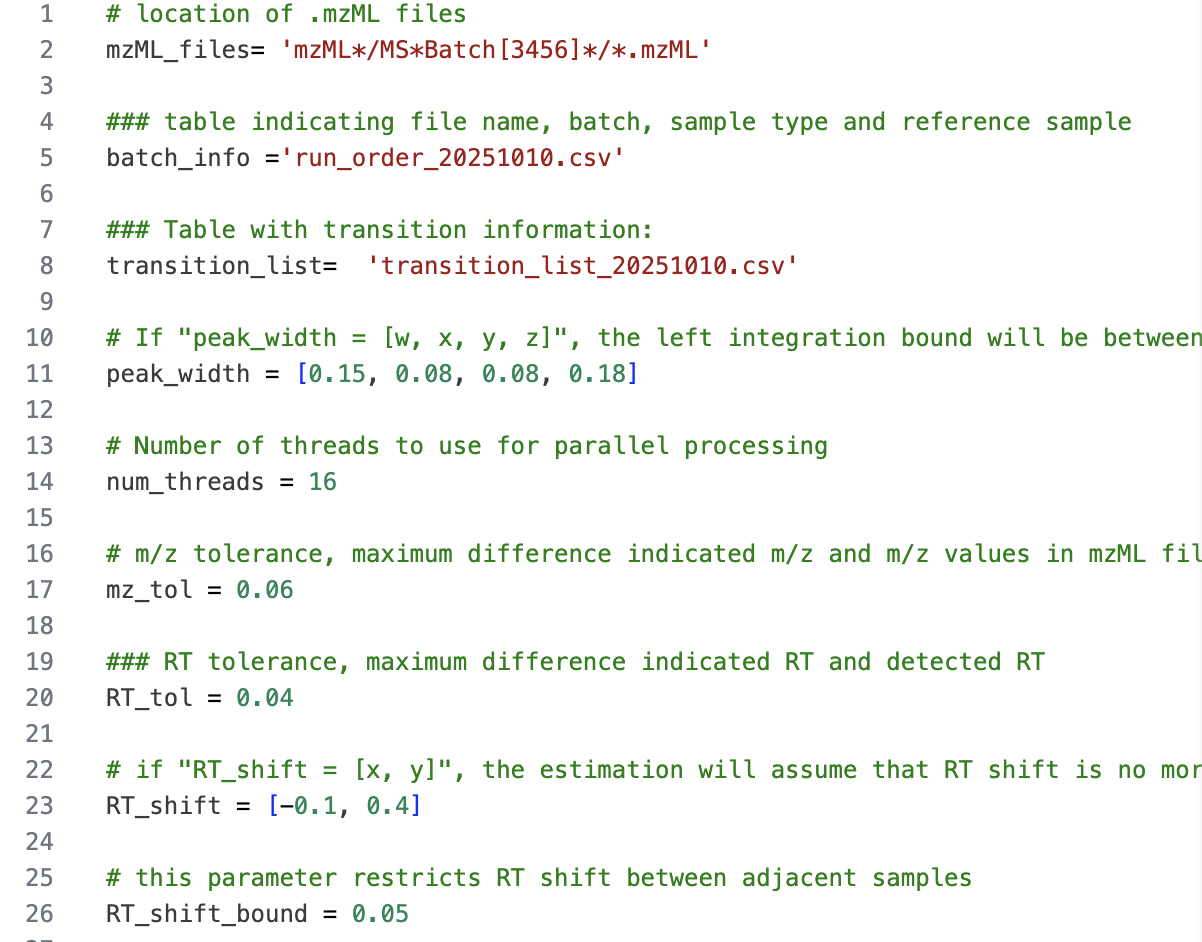
\includegraphics[width=0.7\linewidth,height=\textheight,keepaspectratio]{images/paste-7.png}

}

\caption{\textbf{Global settings file (param.txt).} Screenshot of the
param.txt file used for this dataset, showing all configured parameters
and their values.}

\end{figure}%

\paragraph{Sample Table}\label{sample-table}

In the sample table (run\_order\_20251009.csv) the samples to be
processed were listed by their .mzML file names. The first two BQC
(batch quality control) samples were selected as retention time
reference anchors. The sample type for each sample was defined in column
C (sample\_type) using the
\href{https://slinghub.github.io/MRMhub/articles/02_keydataids.html\#qc-types-sample-types}{MRMhub
QC type} nomenclature. This is optional and INTEGRATOR distinguishes
only between blanks (identified by the presence of the text
\texttt{BLK}), and non-blanks.

\begin{figure}[H]

{\centering 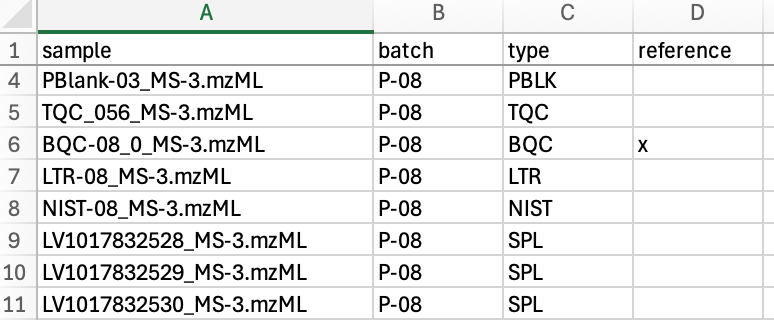
\includegraphics[width=0.5\linewidth,height=\textheight,keepaspectratio]{images/paste-8.png}

}

\caption{Sample Table. Screenshot of a portion of the CSV file used for
this dataset (run\_order\_20251010.csv).}

\end{figure}%

\paragraph{Feature/Transition (Feature)
Table}\label{featuretransition-feature-table}

The feature/transition table (transition\_list\_20251010.csv) defined
the transitions to be extracted from the .mzML files by precursor and
product m/z values. Each feature (peak or peak group) was specified by
its expected retention time (RT, in minutes). For some transitions,
multiple features were defined. The corresponding internal standard
feature for each entry was included in the table, however, these
internal standards were not used by INTEGRATOR but were exported in the
integration results.

\begin{figure}[H]

{\centering 
\includegraphics[width=0.75\linewidth,height=\textheight,keepaspectratio]{data/dataset-3/images/paste-6.png}

}

\caption{\textbf{Feature/Transition Table}. Screenshot of a portion of
the CSV file (transition\_list\_20251010\_Final.csv) used for this
dataset. Feature-specific peak widths and fixed integration borders were
set for three adjacent features to ensure correct integration.}

\end{figure}%

Feature-specific `peak\_width' settings were applied for multiple
features in this dataset when peaks were broader, exhibited increased
tailing, or consisted of convoluted peaks that had to be co-integrated
(see Figure 4 a-d). Fixed borders were assigned for features for which
automatic integration failed or produced inconsistent results due to
being poorly separated from adjacent peaks or having noisy, and
consequently were applied when necessary (see Figure 4 e-h). The final
version of the feature/transition table (transition\_list\_20251010.csv)
is the result from several rounds of parameter optimization with
INTEGRATOR.

\begin{figure}[H]

{\centering 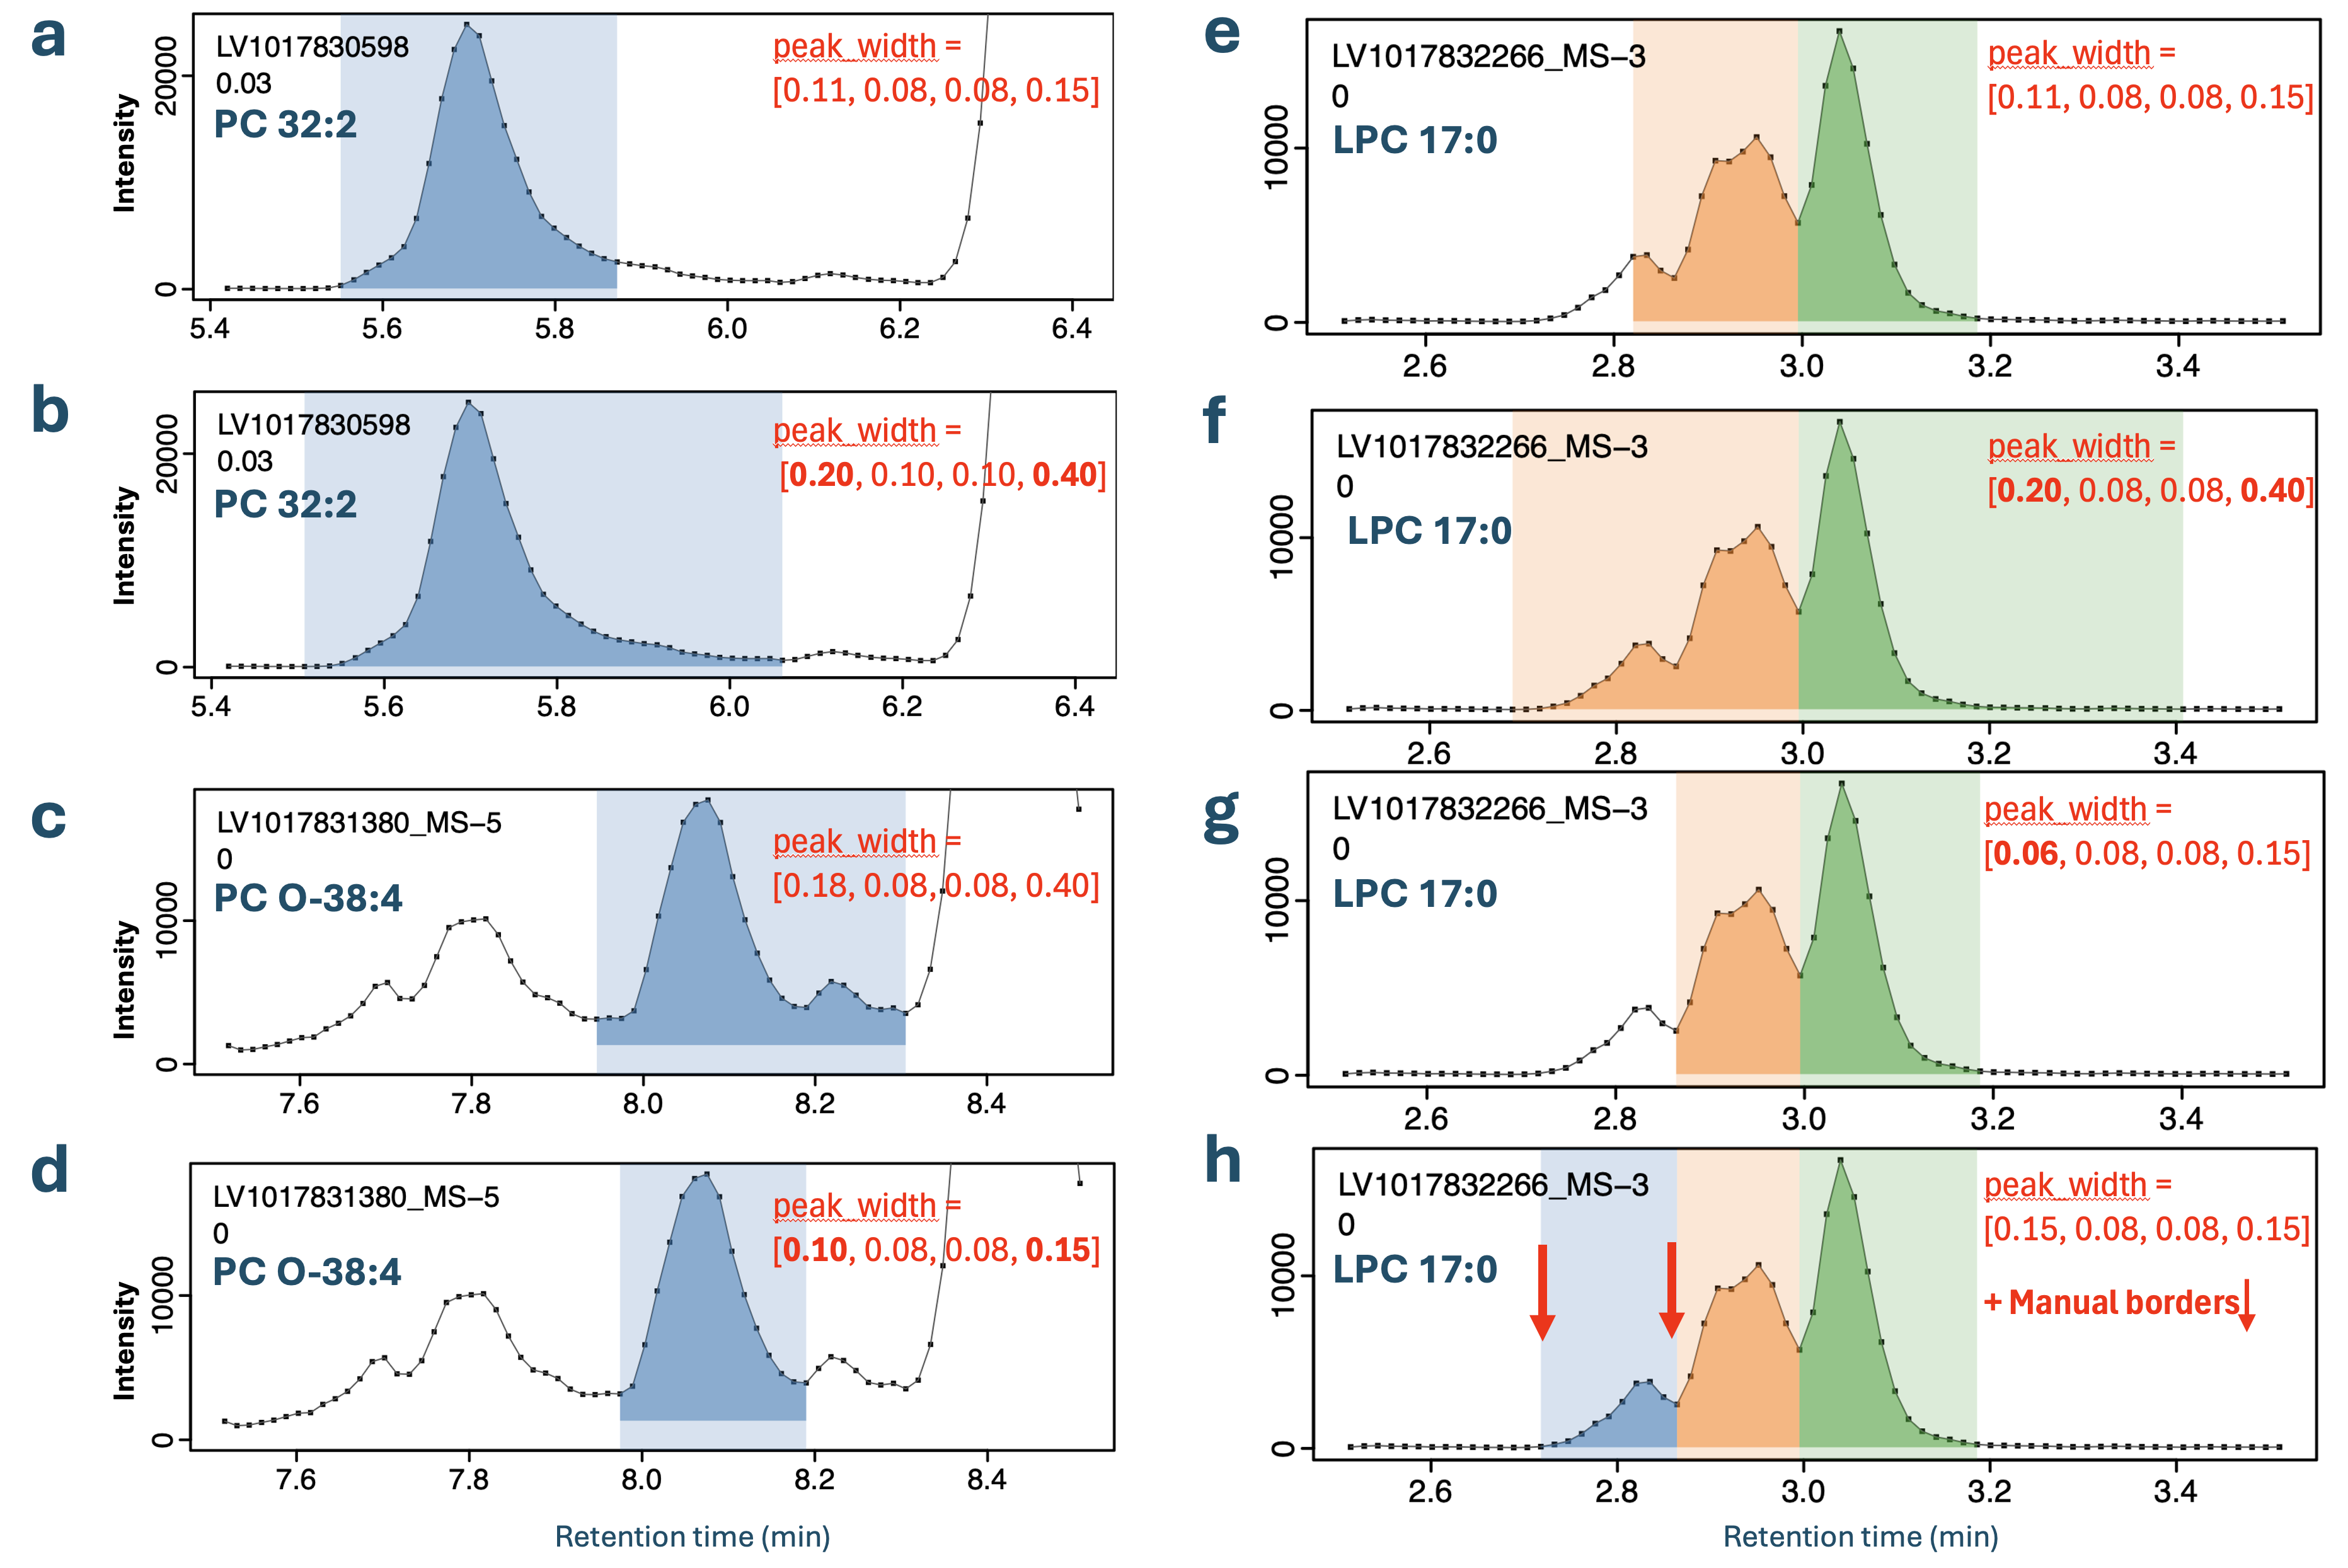
\includegraphics[width=1\linewidth,height=\textheight,keepaspectratio]{images/paste-9.png}

}

\caption{\textbf{Examples of manually set peak boundaries for
MRMhub-INTEGRATOR.} (a, b) The effect of different peak\_width parameter
settings on the integration of a peak with clear tailing (PC 36:6).
Panel (a) displays the result using the global setting, which is
suitable for the majority of peaks. Panel (b) shows the outcome of
applying a feature-specific peak width setting that overrides the global
parameter for improved integration. (c, d) The influence of the
peak\_width parameter on the integration of a peak with nearby
interferences (PC O-38:4). Panel (c) corresponds to the global setting,
whereas panel (d) illustrates how an excessively wide peak border
setting can cause incorrect integration, emphasizing the importance of
establishing a suitable global value. (e, f) The effect of various peak
integration settings on a complex chromatogram containing overlapping
peaks. The global setting, shown in Panel (e), leads to partial
integration where the first peak is not correctly recognized. While
adjusting the peak width to be too relaxed resulted in the inclusion of
the entire interfering signal and a more narrow setting led to its
exclusion, neither was optimal. The final configuration, shown in Panel
(f), used fixed boundaries defined for the first peak, which allowed for
the correct picking and integration of all three isomer peaks of LPC
17:0.}

\end{figure}%

\subsection{Running MRMhub-INTEGRATOR and Review of
Results}\label{running-mrmhub-integrator-and-review-of-results}

The most recent release OF INTEGRATOR was obtained from
\url{https://github.com/SLINGhub/MRMhub/releases}. After preparing all
input files, the mrmhub application is started. Steps 1 to 4 then run
consecutively without further input to perform peak detection, peak
picking, integration, and export of data and PDF results. The
integration results are reported in the generated file `long.csv', a
long-format table that includes peak areas, actual retention time, peak
width, and other metadata. This data file will be used for subsequent
data postprocessing (see the following section). A wide-format table
with peak areas is available as `quant\_raw.csv'. PDFs of the integrated
transitions are available in the by\_* folders. See the
\hyperref[0]{INTEGRATOR Manual} for more details.

The peak integration results were inspected for all features across
samples using the generated PDFs (see above). In this dataset, RT shifts
across the entire run of 4,591 samples were less than 0.04 min, except
for \textasciitilde{} 20 samples at the start of a batch towards the end
of this analysis, which had increased RT shifts.

\begin{figure}[H]

{\centering 
\includegraphics[width=0.62\linewidth,height=\textheight,keepaspectratio]{data/dataset-3/images/paste-3.png}

}

\caption{MRMhub-INTEGRATOR application.}

\end{figure}%

\section{Data Postprocessing and QC}\label{data-postprocessing-and-qc}

\subsection{Setting up a Quarto Notebook and Installation of
\{mrmhub\}}\label{setting-up-a-quarto-notebook-and-installation-of-mrmhub}

A \href{https://quarto.org/}{Quarto} notebook was created in
\href{https://posit.co/download/rstudio-desktop/}{RStudio} the
\{mrmhub\} R package was installed by running following code in the R
console, which also installs two other R packages used in this workflow.

\begin{Shaded}
\begin{Highlighting}[]
\ControlFlowTok{if}\NormalTok{ (}\SpecialCharTok{!}\FunctionTok{require}\NormalTok{(}\StringTok{"remotes"}\NormalTok{)) }\FunctionTok{install.packages}\NormalTok{(}\StringTok{"remotes"}\NormalTok{)}
\NormalTok{remotes}\SpecialCharTok{::}\FunctionTok{install\_github}\NormalTok{(}\StringTok{"SLINGhub/MRMhub"}\NormalTok{, }\AttributeTok{subdir =} \StringTok{"quant"}\NormalTok{)}
\FunctionTok{install.packages}\NormalTok{(}\StringTok{"here"}\NormalTok{) }\CommentTok{\# Used for parallel processing}
\end{Highlighting}
\end{Shaded}

The Quarto notebook code generated in this example workflow is available
from \url{https://github.com/SLINGhub/MRMhub-workflows} (file
Dataset3.qmd). In the subsequent section, the data postprocessing is
encoded and documented step-by-step into the notebook as individual code
chunks using \{mrmhub\} functions. Certain code chunks include
additional R code to showcase specific examples for illustrative
purposes. In real-world applications, this supplementary may not be
necessary.

\subsection{Postprocessing workflow}\label{postprocessing-workflow}

\subsubsection{\texorpdfstring{Load \texttt{mrmhub} and other required R
packages}{Load mrmhub and other required R packages}}\label{load-mrmhub-and-other-required-r-packages}

To improve performance multi-threading was used for some of the
calculations and plottings, for which the R package \{mirai\} needs to
be installed and loaded.

\begin{Shaded}
\begin{Highlighting}[]
\FunctionTok{library}\NormalTok{(mrmhub)}
\FunctionTok{library}\NormalTok{(mirai)  }\CommentTok{\# Used for parallel processing}
\end{Highlighting}
\end{Shaded}

\subsubsection{Import the MRMhub-INTEGRATOR
results}\label{import-the-mrmhub-integrator-results}

The results from the peak integration performed with the INTEGRATOR
workflow, as described in the previous section, were imported into a
\texttt{MRMhubExperiment} data object. This object represents the
central data container used in this postprocessing workflow. Nogte that
the original result file from INTEGRATOR (`long.csv') has been renamed
to `Dataset3\_MRMhub-Integrator\_20251010.csv'

\begin{Shaded}
\begin{Highlighting}[]
\NormalTok{data\_path }\OtherTok{\textless{}{-}} \StringTok{"./data/dataset{-}3/data/Dataset3\_MRMhub{-}Integrator\_20251010.csv"}
\NormalTok{mexp }\OtherTok{\textless{}{-}} \FunctionTok{MRMhubExperiment}\NormalTok{()}
\NormalTok{mexp }\OtherTok{\textless{}{-}} \FunctionTok{import\_data\_mrmhub}\NormalTok{(mexp, data\_path, }\AttributeTok{import\_metadata =} \ConstantTok{TRUE}\NormalTok{)                        }
\CommentTok{\#\textgreater{} v Imported 4591 analyses with 828 features}
\CommentTok{\#\textgreater{} i \textasciigrave{}feature\_area\textasciigrave{} selected as default feature intensity. Modify with \textasciigrave{}set\_intensity\_var()\textasciigrave{}.}
\CommentTok{\#\textgreater{} v Analysis metadata associated with 4591 analyses.}
\CommentTok{\#\textgreater{} v Feature metadata associated with 828 features.}
\end{Highlighting}
\end{Shaded}

\subsubsection{Import the analysis
metadata}\label{import-the-analysis-metadata}

Detailed analysis metadata, describing the analytes, samples, features,
internal standards (ISTDs), and response curves required for subsequent
steps, were imported from the Excel workbook
`Dataset3\_Metadata\_20251010.xlsm'. This workbook is available within
the previously mentioned Zenodo archive (record Dataset 3).

\begin{Shaded}
\begin{Highlighting}[]
\NormalTok{file\_path }\OtherTok{\textless{}{-}} \StringTok{"./data/dataset{-}3/data/Dataset3\_Metadata\_20251010.xlsm"}
\NormalTok{mexp }\OtherTok{\textless{}{-}} \FunctionTok{import\_metadata\_msorganiser}\NormalTok{(mexp, file\_path, }\AttributeTok{ignore\_warnings =} \ConstantTok{TRUE}\NormalTok{)}
\CommentTok{\#\textgreater{} ! Metadata has following warnings and notifications:}
\CommentTok{\#\textgreater{} {-}{-}{-}{-}{-}{-}{-}{-}{-}{-}{-}{-}{-}{-}{-}{-}{-}{-}{-}{-}{-}{-}{-}{-}{-}{-}{-}{-}{-}{-}{-}{-}{-}{-}{-}{-}{-}{-}{-}{-}{-}{-}{-}{-}{-}{-}{-}{-}{-}{-}{-}{-}{-}{-}{-}{-}{-}{-}{-}{-}{-}{-}{-}{-}{-}{-}{-}{-}{-}{-}{-}{-}{-}{-}{-}{-}{-}{-}{-}{-}{-}{-}{-}{-}{-}{-}{-}{-}{-}{-}{-}{-}}
\CommentTok{\#\textgreater{}   Type Table    Column     Issue                           Count}
\CommentTok{\#\textgreater{} 1 W*   Features feature\_id Feature(s) not in analysis data    31}
\CommentTok{\#\textgreater{} 2 W*   Features feature\_id Feature(s) without metadata         1}
\CommentTok{\#\textgreater{} {-}{-}{-}{-}{-}{-}{-}{-}{-}{-}{-}{-}{-}{-}{-}{-}{-}{-}{-}{-}{-}{-}{-}{-}{-}{-}{-}{-}{-}{-}{-}{-}{-}{-}{-}{-}{-}{-}{-}{-}{-}{-}{-}{-}{-}{-}{-}{-}{-}{-}{-}{-}{-}{-}{-}{-}{-}{-}{-}{-}{-}{-}{-}{-}{-}{-}{-}{-}{-}{-}{-}{-}{-}{-}{-}{-}{-}{-}{-}{-}{-}{-}{-}{-}{-}{-}{-}{-}{-}{-}{-}{-}}
\CommentTok{\#\textgreater{} E = Error, W = Warning, W* = Supressed Warning, N = Note}
\CommentTok{\#\textgreater{} {-}{-}{-}{-}{-}{-}{-}{-}{-}{-}{-}{-}{-}{-}{-}{-}{-}{-}{-}{-}{-}{-}{-}{-}{-}{-}{-}{-}{-}{-}{-}{-}{-}{-}{-}{-}{-}{-}{-}{-}{-}{-}{-}{-}{-}{-}{-}{-}{-}{-}{-}{-}{-}{-}{-}{-}{-}{-}{-}{-}{-}{-}{-}{-}{-}{-}{-}{-}{-}{-}{-}{-}{-}{-}{-}{-}{-}{-}{-}{-}{-}{-}{-}{-}{-}{-}{-}{-}{-}{-}{-}{-}}
\CommentTok{\#\textgreater{} v Analysis metadata associated with 4591 analyses.}
\CommentTok{\#\textgreater{} v Feature metadata associated with 827 features.}
\CommentTok{\#\textgreater{} v Internal Standard metadata associated with 26 ISTDs.}
\CommentTok{\#\textgreater{} v Response curve metadata associated with 36 annotated analyses.}
\end{Highlighting}
\end{Shaded}

\subsubsection{Analytical design and
timeline}\label{analytical-design-and-timeline}

An overview of the analysis structure, detailing the types and sequence
of QC samples analyzed is provided by the plot below. It also shows
information on the start and end dates, total duration, and median run
time for each sample. Setting \texttt{show\_timestamp\ =\ TRUE} in the
code below will plot the absolute dates as the x-axis, showing three
short interruptions, and the last 4 batches were measured approximately
one year later.

\begin{Shaded}
\begin{Highlighting}[]
\FunctionTok{plot\_runsequence}\NormalTok{(}
\NormalTok{  mexp, }
  \AttributeTok{show\_batches =} \ConstantTok{TRUE}\NormalTok{, }
  \AttributeTok{qc\_types =} \FunctionTok{c}\NormalTok{(}\StringTok{"SPL"}\NormalTok{, }\StringTok{"BQC"}\NormalTok{, }\StringTok{"TQC"}\NormalTok{, }\StringTok{"PBLK"}\NormalTok{, }\StringTok{"UBLK"}\NormalTok{, }\StringTok{"RQC"}\NormalTok{, }\StringTok{"SBLK"}\NormalTok{, }\StringTok{"LTR"}\NormalTok{, }\StringTok{"NIST"}\NormalTok{),}
  \AttributeTok{batch\_zebra\_stripe =} \ConstantTok{TRUE}\NormalTok{, }\AttributeTok{base\_font\_size =} \DecValTok{6}\NormalTok{,}
  \AttributeTok{batch\_fill\_color =} \StringTok{"\#fffbdb"}\NormalTok{, }
  \AttributeTok{segment\_linewidth =} \FloatTok{0.25}\NormalTok{,}
  \AttributeTok{show\_timestamp =} \ConstantTok{FALSE}\NormalTok{) }\SpecialCharTok{+}
  \FunctionTok{theme}\NormalTok{(}\AttributeTok{plot.title =} \FunctionTok{element\_text}\NormalTok{(}\AttributeTok{size =} \DecValTok{5}\NormalTok{))}
\end{Highlighting}
\end{Shaded}

\includegraphics[width=1\linewidth,height=\textheight,keepaspectratio]{Dataset3_files/figure-pdf/chunk6-runsequence-1.pdf}

\subsubsection{Overview Chromatographic
Separation}\label{overview-chromatographic-separation}

The following plot shows the retention time distribution of all detected
lipid species. The ceramides (Cer) species show little chromatographic
separation in contrast to other lipid classes, with the majority eluting
between 10.0 to 10.5 min. The triglycerides (TG) also elute within a
narrower retention time range at around 11 min.

\begin{Shaded}
\begin{Highlighting}[]
\FunctionTok{plot\_abundanceprofile}\NormalTok{(}
  \AttributeTok{data =}\NormalTok{ mexp,}
  \AttributeTok{log\_scale =} \ConstantTok{FALSE}\NormalTok{,}
  \AttributeTok{variable =} \StringTok{"rt"}\NormalTok{, }
  \AttributeTok{density\_strip =} \ConstantTok{TRUE}\NormalTok{,}
  \AttributeTok{qc\_types =} \StringTok{"SPL"}\NormalTok{,}
  \AttributeTok{analysis\_range =} \FunctionTok{c}\NormalTok{(}\DecValTok{1}\NormalTok{,}\DecValTok{4000}\NormalTok{),}
  \AttributeTok{show\_sum =} \ConstantTok{FALSE}\NormalTok{,}
  \CommentTok{\#x\_lim = c(6.5, 7.5),}
  \AttributeTok{x\_label =} \ConstantTok{NA}\NormalTok{,}
  \AttributeTok{feature\_map =} \StringTok{"lipidomics"}\NormalTok{)}
\end{Highlighting}
\end{Shaded}

\includegraphics[width=1\linewidth,height=\textheight,keepaspectratio]{Dataset3_files/figure-pdf/chunk6b-rtplot-1.pdf}

\subsubsection{Overall trends and check for possible
outliers}\label{overall-trends-and-check-for-possible-outliers}

To examine overall technical trends and issues affecting most analytes
(features), the Relative Log Abundance (RLA) plot is useful (De Livera
et al., 2015 (Livera et al. 2015)). In an RLA plot, each feature is
normalized to the across-sample or within-batch median and the resulting
values are shown as boxplots for each sample. This visualization helps
identify technical problems such as pipetting errors, sample loss, or
changes in injection volume or instrument sensitivity. First, an
overview of all analyses (runs) is plotted.

First, an overview of all analyses (samples) or samples is plotted,
whereby on the signals from the spiked-in internal standards signals
(ISTDs) are shown. The red horizontal lines indicate 1.5X IQR outlier
limits.

\begin{Shaded}
\begin{Highlighting}[]
\NormalTok{fig2a }\OtherTok{\textless{}{-}} \FunctionTok{plot\_rla\_boxplot}\NormalTok{(}
  \AttributeTok{data =}\NormalTok{ mexp,}
  \AttributeTok{rla\_type\_batch =} \FunctionTok{c}\NormalTok{(}\StringTok{"within"}\NormalTok{),}
  \AttributeTok{variable =} \StringTok{"intensity"}\NormalTok{,}
  \AttributeTok{qc\_types =} \FunctionTok{c}\NormalTok{(}\StringTok{"BQC"}\NormalTok{, }\StringTok{"TQC"}\NormalTok{, }\StringTok{"SPL"}\NormalTok{, }\StringTok{"NIST"}\NormalTok{, }\StringTok{"LTR"}\NormalTok{, }\StringTok{"SBLK"}\NormalTok{),  }
  \CommentTok{\#plot\_range = c(1, 4900),}
  \AttributeTok{rla\_limit\_to\_range =} \ConstantTok{FALSE}\NormalTok{,}
  \AttributeTok{filter\_data =} \ConstantTok{FALSE}\NormalTok{,}
  \AttributeTok{min\_feature\_intensity =} \DecValTok{1000}\NormalTok{,}
  \AttributeTok{include\_feature\_filter =} \StringTok{"ISTD"}\NormalTok{,}
  \CommentTok{\#y\_lim = c({-}4,4),}
  \AttributeTok{show\_timestamp =} \ConstantTok{FALSE}\NormalTok{,}
  \AttributeTok{outlier\_method =} \StringTok{"fold"}\NormalTok{,}
  \AttributeTok{outlier\_k =} \FunctionTok{c}\NormalTok{(}\SpecialCharTok{{-}}\FloatTok{0.4}\NormalTok{, }\FloatTok{0.3}\NormalTok{),}
  \AttributeTok{outlier\_exclude =} \ConstantTok{FALSE}\NormalTok{, }
  \AttributeTok{x\_gridlines =} \ConstantTok{FALSE}\NormalTok{,}
  \AttributeTok{show\_plot =} \ConstantTok{TRUE}\NormalTok{,}
  \AttributeTok{batch\_zebra\_stripe =} \ConstantTok{TRUE}\NormalTok{,}
  \AttributeTok{linewidth =} \FloatTok{0.1}
\NormalTok{)}
\CommentTok{\#\textgreater{} i Found 148 outliers in the 4545 shown analyses}
\end{Highlighting}
\end{Shaded}

\includegraphics[width=1\linewidth,height=\textheight,keepaspectratio]{Dataset3_files/figure-pdf/chunk7-rla-plot_overview-1.pdf}

Several outliers among study and QC samples were detected using this RLA
analysis (visible also in the plot above)

\begin{Shaded}
\begin{Highlighting}[]
\CommentTok{\# Get outlier in ISTD total signal excluding 3 batches with overall lower ISTD}
\NormalTok{istd\_outlier }\OtherTok{\textless{}{-}}\NormalTok{ fig2a}\SpecialCharTok{$}\NormalTok{outliers }\SpecialCharTok{|\textgreater{}} 
  \FunctionTok{filter}\NormalTok{(}\SpecialCharTok{!}\NormalTok{(batch\_id }\SpecialCharTok{\%in\%} \FunctionTok{c}\NormalTok{(}\StringTok{"P{-}01"}\NormalTok{, }\StringTok{"P{-}02"}\NormalTok{, }\StringTok{"P{-}43"}\NormalTok{) }\SpecialCharTok{\&}\NormalTok{ val\_res\_median }\SpecialCharTok{\textgreater{}} \SpecialCharTok{{-}}\DecValTok{3}\NormalTok{))}

\FunctionTok{print}\NormalTok{(istd\_outlier)}
\CommentTok{\#\textgreater{} \# A tibble: 79 x 5}
\CommentTok{\#\textgreater{}    analysis\_id       analysis\_order batch\_id val\_res\_median qc\_type}
\CommentTok{\#\textgreater{}    \textless{}chr\textgreater{}                      \textless{}int\textgreater{} \textless{}chr\textgreater{}             \textless{}dbl\textgreater{} \textless{}chr\textgreater{}  }
\CommentTok{\#\textgreater{}  1 LV1017832619\_MS{-}3            113 P{-}08             {-}11.8  SPL    }
\CommentTok{\#\textgreater{}  2 LV1017835020\_MS{-}3            804 P{-}14             {-}11.8  SPL    }
\CommentTok{\#\textgreater{}  3 BQC{-}18\_0\_MS{-}4               1157 P{-}18              {-}2.69 BQC    }
\CommentTok{\#\textgreater{}  4 LV1017831110\_MS{-}4           1185 P{-}18             {-}11.7  SPL    }
\CommentTok{\#\textgreater{}  5 LV1017832095\_MS{-}4           1213 P{-}18             {-}12.1  SPL    }
\CommentTok{\#\textgreater{}  6 LV1017831999\_MS{-}4           1328 P{-}19             {-}12.0  SPL    }
\CommentTok{\#\textgreater{}  7 LV1017834759\_MS{-}4           1990 P{-}25             {-}11.9  SPL    }
\CommentTok{\#\textgreater{}  8 LV1017834663\_MS{-}5           2218 P{-}27             {-}11.6  SPL    }
\CommentTok{\#\textgreater{}  9 TQC\_217\_MS{-}5                2320 P{-}28             {-}12.0  TQC    }
\CommentTok{\#\textgreater{} 10 TQC\_218\_MS{-}5                2334 P{-}28             {-}12.9  TQC    }
\CommentTok{\#\textgreater{} \# i 69 more rows}
\end{Highlighting}
\end{Shaded}

To confirm these potential outliers, the peak areas of all ISTDs in
different QC types is plotted against the run order (RunScatter plot).
The outliers seen\textbackslash{} in these plots (with values close to
zero) correspond to the outliers seen in the RLA plot above.

\begin{Shaded}
\begin{Highlighting}[]
\FunctionTok{plot\_runscatter}\NormalTok{(mexp, }\AttributeTok{variable =} \StringTok{"intensity"}\NormalTok{, }
                \AttributeTok{include\_qualifier =} \ConstantTok{FALSE}\NormalTok{,}
                \AttributeTok{qc\_types =} \FunctionTok{c}\NormalTok{(}\StringTok{"SPL"}\NormalTok{, }\StringTok{"BQC"}\NormalTok{, }\StringTok{"TQC"}\NormalTok{, }\StringTok{"PBLK"}\NormalTok{, }\StringTok{"RQC"}\NormalTok{, }\StringTok{"SBLK"}\NormalTok{),}
                \AttributeTok{include\_feature\_filter =} \StringTok{"IS"}\NormalTok{,}
                \CommentTok{\#y\_min = 0.00, y\_max = 0.15,}
                \CommentTok{\#plot\_range = c(0, 910),}
                \AttributeTok{point\_size =}\NormalTok{ .}\DecValTok{2}\NormalTok{,}
                \AttributeTok{point\_border\_width =} \FloatTok{0.1}\NormalTok{,}
                \AttributeTok{point\_transparency =}\NormalTok{ .}\DecValTok{7}\NormalTok{,}
                \AttributeTok{base\_font\_size =} \DecValTok{43}\NormalTok{,}
                \AttributeTok{cols\_page =} \DecValTok{3}\NormalTok{,}
                \AttributeTok{rows\_page =} \DecValTok{11}\NormalTok{,}
                \AttributeTok{show\_progress =} \ConstantTok{FALSE}\NormalTok{,}
                \AttributeTok{cap\_outliers =} \ConstantTok{TRUE}\NormalTok{)}
\CommentTok{\#\textgreater{} Generating plots (1 page)}
\end{Highlighting}
\end{Shaded}

\includegraphics[width=1\linewidth,height=\textheight,keepaspectratio]{Dataset3_files/figure-pdf/chunk8-runscatter-plot-istd-1-1.pdf}

Sepatedly, the full dataset is then checked for potential systematic
outliers in endogenous analytes.

\begin{Shaded}
\begin{Highlighting}[]
\NormalTok{fig2b }\OtherTok{\textless{}{-}} \FunctionTok{plot\_rla\_boxplot}\NormalTok{(}
  \AttributeTok{data =}\NormalTok{ mexp,}
  \AttributeTok{rla\_type\_batch =} \FunctionTok{c}\NormalTok{(}\StringTok{"within"}\NormalTok{),}
  \AttributeTok{variable =} \StringTok{"intensity"}\NormalTok{,}
  \AttributeTok{qc\_types =} \FunctionTok{c}\NormalTok{(}\StringTok{"BQC"}\NormalTok{, }\StringTok{"TQC"}\NormalTok{, }\StringTok{"SPL"}\NormalTok{, }\StringTok{"NIST"}\NormalTok{, }\StringTok{"LTR"}\NormalTok{),  }
  \AttributeTok{filter\_data =} \ConstantTok{FALSE}\NormalTok{,}
  \AttributeTok{min\_feature\_intensity =} \DecValTok{1000}\NormalTok{,}
  \AttributeTok{exclude\_feature\_filter =} \StringTok{"ISTD"}\NormalTok{,}
  \AttributeTok{plot\_range =} \FunctionTok{c}\NormalTok{(}\DecValTok{1}\NormalTok{, }\DecValTok{4800}\NormalTok{),}
  \CommentTok{\#y\_lim = c({-}4,4),}
  \AttributeTok{show\_timestamp =} \ConstantTok{FALSE}\NormalTok{,}
  \AttributeTok{outlier\_method =} \StringTok{"fold"}\NormalTok{,}
  \AttributeTok{outlier\_k =} \FunctionTok{c}\NormalTok{(}\SpecialCharTok{{-}}\DecValTok{2}\NormalTok{,}\DecValTok{1}\NormalTok{) ,}
  \AttributeTok{outlier\_exclude =} \ConstantTok{FALSE}\NormalTok{, }
  \AttributeTok{x\_gridlines =} \ConstantTok{FALSE}\NormalTok{,}
  \AttributeTok{batch\_zebra\_stripe =} \ConstantTok{TRUE}\NormalTok{,}
  \AttributeTok{show\_plot =} \ConstantTok{TRUE}\NormalTok{,}
  \AttributeTok{linewidth =} \FloatTok{0.1}
\NormalTok{) }
\CommentTok{\#\textgreater{} i Found 81 outliers in the 4540 shown analyses}
\end{Highlighting}
\end{Shaded}

\includegraphics[width=1\linewidth,height=\textheight,keepaspectratio]{Dataset3_files/figure-pdf/chunk9-rla-plot_overview2-1.pdf}

Also for the endogenous analytes, several outliers among study and QC
samples were detected:

\begin{Shaded}
\begin{Highlighting}[]
\CommentTok{\# Get outlier in ISTD total signal excluding 3 batches with conistently lower ISTD}
\NormalTok{analyte\_outlier }\OtherTok{\textless{}{-}}\NormalTok{ fig2b}\SpecialCharTok{$}\NormalTok{outliers }\SpecialCharTok{|\textgreater{}} 
  \FunctionTok{filter}\NormalTok{(}\SpecialCharTok{!}\NormalTok{(batch\_id }\SpecialCharTok{\%in\%} \FunctionTok{c}\NormalTok{(}\StringTok{"P{-}01"}\NormalTok{, }\StringTok{"P{-}02"}\NormalTok{, }\StringTok{"P{-}43"}\NormalTok{) }\SpecialCharTok{\&}\NormalTok{ val\_res\_median }\SpecialCharTok{\textgreater{}} \SpecialCharTok{{-}}\DecValTok{3}\NormalTok{))}
\FunctionTok{print}\NormalTok{(analyte\_outlier)}
\CommentTok{\#\textgreater{} \# A tibble: 72 x 5}
\CommentTok{\#\textgreater{}    analysis\_id       analysis\_order batch\_id val\_res\_median qc\_type}
\CommentTok{\#\textgreater{}    \textless{}chr\textgreater{}                      \textless{}int\textgreater{} \textless{}chr\textgreater{}             \textless{}dbl\textgreater{} \textless{}chr\textgreater{}  }
\CommentTok{\#\textgreater{}  1 LV1017832619\_MS{-}3            113 P{-}08             {-}10.5  SPL    }
\CommentTok{\#\textgreater{}  2 LV1017835020\_MS{-}3            804 P{-}14              {-}9.91 SPL    }
\CommentTok{\#\textgreater{}  3 BQC{-}18\_0\_MS{-}4               1157 P{-}18              {-}2.29 BQC    }
\CommentTok{\#\textgreater{}  4 LV1017832063\_MS{-}4           1176 P{-}18              {-}9.48 SPL    }
\CommentTok{\#\textgreater{}  5 LV1017831110\_MS{-}4           1185 P{-}18              {-}9.98 SPL    }
\CommentTok{\#\textgreater{}  6 LV1017832095\_MS{-}4           1213 P{-}18             {-}10.0  SPL    }
\CommentTok{\#\textgreater{}  7 LV1017832134\_MS{-}4           1260 P{-}18               1.21 SPL    }
\CommentTok{\#\textgreater{}  8 LV1017831999\_MS{-}4           1328 P{-}19              {-}9.78 SPL    }
\CommentTok{\#\textgreater{}  9 LV1017834759\_MS{-}4           1990 P{-}25              {-}9.82 SPL    }
\CommentTok{\#\textgreater{} 10 LV1017834663\_MS{-}5           2218 P{-}27             {-}10.4  SPL    }
\CommentTok{\#\textgreater{} \# i 62 more rows}
\end{Highlighting}
\end{Shaded}

Inspection of the generated plots and outlier tables identified several
individual study samples, Technical QC (TQC), and Batch QC (BQC) samples
that exhibited markedly lower signals for both internal standards
(ISTDs) and endogenous analytes. TQC samples from two batches showed
similarly reduced signals, while adjacent samples displayed normal
signal levels, suggesting potential issues with sample preparation or
errors in the LC-MS worklist for these specific samples and batches.
Accordingly, these samples were classified as technical outliers and
excluded from subsequent analysis.

Furthermore, in three batches analyzed toward the end of the sequence,
all BQC samples exhibited significant differences in ISTD and analyte
signals, whereas study samples in the same batch presented normal
signals. This pattern is indicative of probable sample preparation
errors affecting these BQCs. Consequently, they were also classified as
technical outliers and excluded from the dataset..

Finally, an additional 18 samples were identified as outliers based on
their endogenous analyte signals, although their ISTD signals remained
comparable to other samples. These discrepancies were attributed to
errors that occurred during the pipetting of sample aliquots into the
extraction tubes.

\begin{Shaded}
\begin{Highlighting}[]
\CommentTok{\# Outliers in analyte but not ISTD signals}
\FunctionTok{setdiff}\NormalTok{(}
\NormalTok{  analyte\_outlier}\SpecialCharTok{$}\NormalTok{analysis\_id,}
\NormalTok{  istd\_outlier}\SpecialCharTok{$}\NormalTok{analysis\_id }
\NormalTok{)}
\CommentTok{\#\textgreater{}  [1] "LV1017832063\_MS{-}4" "LV1017832134\_MS{-}4" "LV1017834496\_MS{-}5"}
\CommentTok{\#\textgreater{}  [4] "LV1017834500\_MS{-}5" "LV1017831025\_MS{-}5" "BQC{-}30\_8\_MS{-}5"    }
\CommentTok{\#\textgreater{}  [7] "BQC{-}31\_0\_MS{-}5"     "LV1017831362\_MS{-}5" "BQC{-}34\_4\_MS{-}5"    }
\CommentTok{\#\textgreater{} [10] "BQC{-}36\_2\_MS{-}5"     "BQC{-}37\_5\_MS{-}5"     "BQC{-}37\_7\_MS{-}5"    }
\CommentTok{\#\textgreater{} [13] "LV1017834075\_MS{-}5" "LV1017832625\_MS{-}5" "LV1017832682\_MS{-}5"}
\CommentTok{\#\textgreater{} [16] "NIST{-}04"           "LV1017830587"      "LV1017830728"}
\end{Highlighting}
\end{Shaded}

In total, 94 analyses/samples were classified as technical outliers and
will be excluded from further analysis.

\begin{Shaded}
\begin{Highlighting}[]
\CommentTok{\# Combined ISTD and analyte outlier}
\NormalTok{outlier\_combined }\OtherTok{\textless{}{-}}\NormalTok{ istd\_outlier }\SpecialCharTok{|\textgreater{}} 
  \FunctionTok{bind\_rows}\NormalTok{(analyte\_outlier) }\SpecialCharTok{|\textgreater{}}
  \FunctionTok{bind\_rows}\NormalTok{(}\FunctionTok{tibble}\NormalTok{(}\AttributeTok{analysis\_id =} \StringTok{"NIST{-}04"}\NormalTok{, }\AttributeTok{qc\_type =} \StringTok{"NIST"}\NormalTok{)) }\SpecialCharTok{|\textgreater{}} 
  \FunctionTok{select}\NormalTok{(}\SpecialCharTok{{-}}\NormalTok{val\_res\_median) }\SpecialCharTok{|\textgreater{}}
  \FunctionTok{distinct}\NormalTok{()}

\NormalTok{outlier\_combined }\SpecialCharTok{|\textgreater{}}\NormalTok{ dplyr}\SpecialCharTok{::}\FunctionTok{count}\NormalTok{(qc\_type)}
\CommentTok{\#\textgreater{} \# A tibble: 5 x 2}
\CommentTok{\#\textgreater{}   qc\_type     n}
\CommentTok{\#\textgreater{}   \textless{}chr\textgreater{}   \textless{}int\textgreater{}}
\CommentTok{\#\textgreater{} 1 BQC        27}
\CommentTok{\#\textgreater{} 2 LTR         3}
\CommentTok{\#\textgreater{} 3 NIST        5}
\CommentTok{\#\textgreater{} 4 SPL        35}
\CommentTok{\#\textgreater{} 5 TQC        28}

\NormalTok{mexp }\OtherTok{\textless{}{-}} \FunctionTok{exclude\_analyses}\NormalTok{(mexp, }\AttributeTok{analyses =}\NormalTok{ outlier\_combined}\SpecialCharTok{$}\NormalTok{analysis\_id, }\AttributeTok{clear\_existing =} \ConstantTok{TRUE}\NormalTok{)}
\CommentTok{\#\textgreater{} i 97 analyses were excluded for downstream processing. Please reprocess data.}
\end{Highlighting}
\end{Shaded}

To check if these identified outliers were removed the ISTDs are plotted
again. The ISTD signals fairly stable in the first 35 batches, then
varied in the subsequent last 4 batches.

\begin{Shaded}
\begin{Highlighting}[]
\FunctionTok{plot\_runscatter}\NormalTok{(mexp, }\AttributeTok{variable =} \StringTok{"intensity"}\NormalTok{, }
                \AttributeTok{include\_qualifier =} \ConstantTok{FALSE}\NormalTok{,}
                \AttributeTok{qc\_types =} \FunctionTok{c}\NormalTok{(}\StringTok{"SPL"}\NormalTok{, }\StringTok{"BQC"}\NormalTok{, }\StringTok{"TQC"}\NormalTok{, }\StringTok{"PBLK"}\NormalTok{, }\StringTok{"RQC"}\NormalTok{, }\StringTok{"SBLK"}\NormalTok{),}
                \AttributeTok{include\_feature\_filter =} \StringTok{"IS"}\NormalTok{,}
                \CommentTok{\#y\_min = 0.00, y\_max = 0.15,}
                \CommentTok{\#plot\_range = c(0, 910),}
                \AttributeTok{point\_size =}\NormalTok{ .}\DecValTok{2}\NormalTok{,}
                \AttributeTok{point\_border\_width =} \FloatTok{0.1}\NormalTok{,}
                \AttributeTok{point\_transparency =}\NormalTok{ .}\DecValTok{7}\NormalTok{,}
                \AttributeTok{base\_font\_size =} \DecValTok{43}\NormalTok{,}
                \AttributeTok{cols\_page =} \DecValTok{3}\NormalTok{,}
                \AttributeTok{rows\_page =} \DecValTok{11}\NormalTok{,}
                \AttributeTok{show\_progress =} \ConstantTok{FALSE}\NormalTok{,}
                \AttributeTok{cap\_outliers =} \ConstantTok{TRUE}\NormalTok{)}
\CommentTok{\#\textgreater{} Generating plots (1 page)}
\end{Highlighting}
\end{Shaded}

\includegraphics[width=1\linewidth,height=\textheight,keepaspectratio]{Dataset3_files/figure-pdf/chunk12-runscatter-plot-istd-2-1.pdf}

\subsection{Peak picking QC}\label{peak-picking-qc}

To check for potential peak picking errors, the retention time (RT) of
lipid features was plotted against the total carbon number and the
number of double bonds in the acyl chains. This dataset was the result
of an iterative process involving data review with QC plots and
curation, which removed detectable annotation errors. Lipid species that
remained flagged as potential misannotations were then manually
inspected in the chromatograms and compared with an online resource
providing peak annotation information for the utilized LC-MS method
(\url{https://metabolomics.baker.edu.au/method/lipids}). Following this
verification, these features were deemed likely to be correct.

\begin{Shaded}
\begin{Highlighting}[]
\FunctionTok{plot\_rt\_vs\_chain}\NormalTok{(}
\NormalTok{  mexp, }
  \AttributeTok{qc\_types =} \StringTok{"SPL"}\NormalTok{, }
  \AttributeTok{x\_var =} \StringTok{"total\_c"}\NormalTok{, }\AttributeTok{outlier\_residual\_min =} \FloatTok{0.3}\NormalTok{,}
  \AttributeTok{base\_font\_size =} \DecValTok{6}\NormalTok{, }
  \AttributeTok{cols\_page =} \DecValTok{4}\NormalTok{,}
  \AttributeTok{point\_size =} \DecValTok{1}\NormalTok{) }\SpecialCharTok{+}
  \FunctionTok{theme}\NormalTok{( }
    \AttributeTok{legend.position =} \StringTok{"right"}\NormalTok{,}
    \AttributeTok{legend.direction =} \StringTok{"vertical"}\NormalTok{, }
    \AttributeTok{legend.text =} \FunctionTok{element\_text}\NormalTok{(}\AttributeTok{size =}\NormalTok{ base\_font\_size}\SpecialCharTok{*}\FloatTok{0.8}\NormalTok{),}
    \AttributeTok{legend.title =} \FunctionTok{element\_text}\NormalTok{(}\AttributeTok{size =}\NormalTok{ base\_font\_size}\SpecialCharTok{*}\FloatTok{0.8}\NormalTok{),}
    \AttributeTok{legend.key.size =} \FunctionTok{unit}\NormalTok{(base\_font\_size }\SpecialCharTok{*}\FloatTok{0.8}\NormalTok{, }\StringTok{"pt"}\NormalTok{),}
    \AttributeTok{legend.position.inside =} \FunctionTok{c}\NormalTok{(}\FloatTok{0.1}\NormalTok{, }\FloatTok{0.7}\NormalTok{)}
\NormalTok{ )  }
\CommentTok{\#\textgreater{} ! The names of 8 of 827 feature\_id(s) could not be parsed: PDMS{-}10 [+NH4], PDMS{-}11 [+NH4], PDMS{-}12 [+NH4], PDMS{-}13 [+NH4], PDMS{-}14 [+NH4], PDMS{-}15 [+NH4], PDMS{-}16 [+NH4], Ubiquinone.}
\CommentTok{\#\textgreater{} i The following features were flagged as potential annotation outliers: Cer(d18:0/08:0) (ISTD), Cer(d20:1/26:0), Cer(d18:1/19:0), Cer(d18:1/19:0) [{-}H2O], Cer(d18:1/12:0) (ISTD), Cer(d18:2/14:0), DG 36:4 [NL{-}20:4], DG 38:6 [NL{-}22:6], Hex2Cer(d18:1/24:0), Hex1Cer(d18:1/25:0), Hex1Cer(d18:1/24:0), Hex1Cer(d18:1/16:1), PC 40:4 (a), PE 40:4 (a), PE(P{-}18:1/20:3) (a), PE(P{-}18:0/22:5) (b), PE(P{-}18:1/22:5) (a), SM 42:0, SM 40:0, SM 44:1, SM 43:1, SM 40:1, SM 40:1 (d18:1/22:0), SM 35:1 (d18:1/17:0) (a), SM 30:1 (ISTD), SM 44:2, SM 42:2 (b)}
\end{Highlighting}
\end{Shaded}

\includegraphics[width=1\linewidth,height=\textheight,keepaspectratio]{Dataset3_files/figure-pdf/chunk13-peakpickingqc-1.pdf}

\subsection{Feature correlation
analysis}\label{feature-correlation-analysis}

Feature correlation analysis was performed as an additional check for
potential peak annotation errors. In this analysis, feature pairs
exhibiting high correlation (Pearson's r \textgreater{} 0.98), based on
their raw peak areas, were visualized using scatter plots.

\begin{Shaded}
\begin{Highlighting}[]
\CommentTok{\# this below is to exclude a sample that has a very low intensity for all features, see next steps for }
\CommentTok{\# details}
\FunctionTok{plot\_feature\_correlations}\NormalTok{(}
\NormalTok{  mexp, }
  \AttributeTok{variable =} \StringTok{"intensity"}\NormalTok{ , }
  \AttributeTok{qc\_types =} \FunctionTok{c}\NormalTok{(}\StringTok{"SPL"}\NormalTok{, }\StringTok{"BQC"}\NormalTok{, }\StringTok{"TQC"}\NormalTok{), }
  \AttributeTok{point\_size =} \FloatTok{0.5}\NormalTok{, }
  \AttributeTok{cor\_min =} \FloatTok{0.98}\NormalTok{,}
  \AttributeTok{point\_stroke =} \FloatTok{0.1}\NormalTok{,}
  \AttributeTok{sort\_by\_corr =} \ConstantTok{TRUE}\NormalTok{, }
  \AttributeTok{return\_plot =} \ConstantTok{TRUE}\NormalTok{,}
  \AttributeTok{show\_progress =} \ConstantTok{FALSE}\NormalTok{,}
  \AttributeTok{log\_scale =} \ConstantTok{TRUE}\NormalTok{, }
  \AttributeTok{cols\_page =} \DecValTok{5}\NormalTok{, }
  \AttributeTok{rows\_page =} \DecValTok{6}\NormalTok{, }
  \AttributeTok{font\_base\_size =} \DecValTok{5}\NormalTok{)}
\CommentTok{\#\textgreater{} Generating plots (1 page)}
\CommentTok{\#\textgreater{} [[1]]}
\end{Highlighting}
\end{Shaded}

\includegraphics[width=1\linewidth,height=\textheight,keepaspectratio]{Dataset3_files/figure-pdf/chunk14-feature-correlation-1.pdf}

A high correlation (r = 0.986) was observed between features from
unrelated classes, namely SM 39:1 and PC O-36:1. As such a strong
correlation between unrelated species is highly improbable, this was
presumed to be a likely technical or data annotation artefact.
Investigation revealed that these features had overlapping retention
times, and the M+1 isotope of SM 39:1 shared the same transition as PC
O-36:1. A retention time analysis, confirmed with the previously
mentioned online resource, indicated that PC O-36:1 should elute after
SM 39:1. However, the peak corresponding to PC O-36:1 was found at the
end of the MRM window and was partially truncated, which likely
contributed to a peak picking error. Due to this truncation of the PC
O-36:1 peak, this feature was excluded from subsequent analysis.

\begin{Shaded}
\begin{Highlighting}[]
\NormalTok{mexp }\OtherTok{\textless{}{-}} \FunctionTok{exclude\_features}\NormalTok{(mexp, }\AttributeTok{features =} \StringTok{"PC(O{-}36:1)"}\NormalTok{, }\AttributeTok{clear\_existing =} \ConstantTok{TRUE}\NormalTok{)}
\CommentTok{\#\textgreater{} i 1 features were excluded for downstream processing. Please reprocess data.}
\end{Highlighting}
\end{Shaded}

\subsection{Summing up LysoPL and DG
isomers}\label{summing-up-lysopl-and-dg-isomers}

Highly correlating feature pairs from above analysis were found to
consist of numerous lysophospholipid (lyso-PL) sn-1/sn-2 isomers and
diacylglycerol (DG) isomer peaks. This is an expected observation, as
spontaneous positional isomerization, or acyl migration, is known to
occur in vitro during sample preparation and storage (Okudaira et al., J
Lipid Research, 2014 (Okudaira et al. 2014)). Therefore, lyso-PL and DG
isomer pairs were summed into a single feature before subsequent
processing.

\begin{Shaded}
\begin{Highlighting}[]
\NormalTok{mexp }\OtherTok{\textless{}{-}} \FunctionTok{data\_sum\_features}\NormalTok{(mexp, }\AttributeTok{feature\_classes =} \FunctionTok{c}\NormalTok{(}\StringTok{"LPC"}\NormalTok{, }\StringTok{"LPE"}\NormalTok{, }\StringTok{"LPG"}\NormalTok{, }\StringTok{"LPI"}\NormalTok{, }\StringTok{"LPS"}\NormalTok{, }\StringTok{"DG"}\NormalTok{))}
\end{Highlighting}
\end{Shaded}

\subsection{PCA to check for potential technical
outliers}\label{pca-to-check-for-potential-technical-outliers}

To obtain an overview of the data and to perform an additional check for
potential outlier samples, a Principal Component Analysis (PCA) was
conducted based on the raw peak areas of all detected features. The
results show that the BQC samples cluster within the study samples,
whereas the TQC samples form a distinct group. Closer inspection reveals
that TQCs from the last four batches are separated from the other TQCs.
Many samples from these same batches are also found in the lower-left
area of the plot, outside the bulk of the sample points. Furthermore,
BQCs located outside of the main BQC cluster were observed, which are
primarily from batches P-30 to P-38.

\begin{Shaded}
\begin{Highlighting}[]
\FunctionTok{plot\_pca}\NormalTok{(}
  \AttributeTok{data =}\NormalTok{ mexp,}
  \AttributeTok{variable =} \StringTok{"intensity"}\NormalTok{,}
  \AttributeTok{filter\_data =} \ConstantTok{FALSE}\NormalTok{,}
  \AttributeTok{pca\_dims =} \FunctionTok{c}\NormalTok{(}\DecValTok{1}\NormalTok{,}\DecValTok{2}\NormalTok{),}
  \AttributeTok{labels\_threshold\_mad =} \DecValTok{5}\NormalTok{,}
  \AttributeTok{labels\_column =} \StringTok{"analysis\_order"}\NormalTok{,}
  \AttributeTok{qc\_types =} \FunctionTok{c}\NormalTok{(}\StringTok{"BQC"}\NormalTok{, }\StringTok{"TQC"}\NormalTok{, }\StringTok{"LTR"}\NormalTok{, }\StringTok{"NIST"}\NormalTok{, }\StringTok{"SPL"}\NormalTok{),}
  \AttributeTok{ellipse\_variable =} \StringTok{"qc\_type"}\NormalTok{,}
  \AttributeTok{log\_transform =} \ConstantTok{TRUE}\NormalTok{,}\AttributeTok{shared\_labeltext\_hide =} \StringTok{"\_MS{-}5"}\NormalTok{,}
  \AttributeTok{point\_size =} \FloatTok{0.7}\NormalTok{, }\AttributeTok{point\_alpha =} \FloatTok{0.7}\NormalTok{, }\AttributeTok{font\_base\_size =} \DecValTok{8}\NormalTok{, }\AttributeTok{ellipse\_alpha =} \FloatTok{0.3}\NormalTok{,}
  \AttributeTok{include\_istd =} \ConstantTok{FALSE}\NormalTok{,}\AttributeTok{show\_labels =} \ConstantTok{TRUE}\NormalTok{,}\AttributeTok{label\_font\_size =} \FloatTok{1.5}\NormalTok{)   }\SpecialCharTok{+} \FunctionTok{theme}\NormalTok{(}
    \AttributeTok{plot.title =} \FunctionTok{element\_blank}\NormalTok{(),}
    \AttributeTok{aspect.ratio =} \DecValTok{1}\NormalTok{,}
        \AttributeTok{legend.position =} \StringTok{"inside"}\NormalTok{,}
      \AttributeTok{legend.direction =} \StringTok{"vertical"}\NormalTok{, }
      \AttributeTok{legend.text =} \FunctionTok{element\_text}\NormalTok{(}\AttributeTok{size =} \DecValTok{9}\SpecialCharTok{*}\FloatTok{0.7}\NormalTok{),}
      \AttributeTok{legend.title =} \FunctionTok{element\_text}\NormalTok{(}\AttributeTok{size =} \DecValTok{9}\SpecialCharTok{*}\FloatTok{0.7}\NormalTok{),}
      \AttributeTok{legend.key.size =} \FunctionTok{unit}\NormalTok{(}\DecValTok{7} \SpecialCharTok{*}\FloatTok{0.7}\NormalTok{, }\StringTok{"pt"}\NormalTok{),}
      \AttributeTok{legend.position.inside =} \FunctionTok{c}\NormalTok{(}\FloatTok{0.83}\NormalTok{, }\FloatTok{0.83}\NormalTok{)) }
\CommentTok{\#\textgreater{} ! 66 features contained missing or non{-}numeric values and were exluded.}
\CommentTok{\#\textgreater{} i The PCA was calculated based on \textasciigrave{}feature\_intensity\textasciigrave{} values of 741 features.}
\end{Highlighting}
\end{Shaded}

\includegraphics[width=1\linewidth,height=\textheight,keepaspectratio]{Dataset3_files/figure-pdf/chunk17-pca-plot-1.pdf}

The loadings of the principal components (PC) revealed which features
contribute to the variability in the data. While PC1 was contributed to
by many features at similar levels, PC2 showed high loadings for
numerous lyso-PC species. This may indicate systematic effects during
sample preparation and/or analysis that specifically affected this class
of lipids.

\begin{Shaded}
\begin{Highlighting}[]
\FunctionTok{plot\_pca\_loading}\NormalTok{(}
  \AttributeTok{data =}\NormalTok{ mexp,}
  \AttributeTok{variable =} \StringTok{"feature\_intensity"}\NormalTok{,}
  \AttributeTok{include\_istd =} \ConstantTok{FALSE}\NormalTok{,}
  \AttributeTok{pca\_dims =} \FunctionTok{c}\NormalTok{(}\DecValTok{1}\NormalTok{,}\DecValTok{2}\NormalTok{,}\DecValTok{3}\NormalTok{,}\DecValTok{4}\NormalTok{),}
  \AttributeTok{top\_n =} \DecValTok{70}\NormalTok{,}
  \AttributeTok{font\_base\_size =} \DecValTok{7}\NormalTok{,}
  \CommentTok{\#qc\_types = c("SPL", "BQC", "TQC", "LTR"),}
  \AttributeTok{log\_transform =} \ConstantTok{TRUE}\NormalTok{,}
  \CommentTok{\#point\_size = 1, point\_alpha = 0.7, font\_base\_size = 8, ellipse\_alpha = 0.3,}
  \CommentTok{\#include\_istd = FALSE,}
  \CommentTok{\#show\_labels = TRUE,label\_font\_size = 2,}
  \CommentTok{\#shared\_labeltext\_hide = NA}
\NormalTok{  )   }\SpecialCharTok{+} \FunctionTok{theme}\NormalTok{(}
      \AttributeTok{plot.title =} \FunctionTok{element\_blank}\NormalTok{(),}
      \AttributeTok{legend.position =} \StringTok{"inside"}\NormalTok{,}
      \AttributeTok{legend.direction =} \StringTok{"vertical"}\NormalTok{, }
      \AttributeTok{legend.text =} \FunctionTok{element\_text}\NormalTok{(}\AttributeTok{size =} \DecValTok{8}\SpecialCharTok{*}\FloatTok{0.7}\NormalTok{),}
      \AttributeTok{legend.title =} \FunctionTok{element\_text}\NormalTok{(}\AttributeTok{size =} \DecValTok{8}\SpecialCharTok{*}\FloatTok{0.7}\NormalTok{),}
      \AttributeTok{legend.key.size =} \FunctionTok{unit}\NormalTok{(}\DecValTok{6} \SpecialCharTok{*}\FloatTok{0.7}\NormalTok{, }\StringTok{"pt"}\NormalTok{),}
      \AttributeTok{legend.position.inside =} \FunctionTok{c}\NormalTok{(}\FloatTok{0.96}\NormalTok{, }\FloatTok{0.06}\NormalTok{)) }
\end{Highlighting}
\end{Shaded}

\includegraphics[width=1\linewidth,height=\textheight,keepaspectratio]{Dataset3_files/figure-pdf/chunk18-pca-loadings-1.pdf}

\subsection{Matrix effects}\label{matrix-effects}

To assess potential matrix effects arising from differences between
individual samples, the signal distributions of the internal standards
(ISTDs) were plotted for each sample type. The signals correspond to the
median of batch-wise normalized signals. Cholesterol and the
triglyceride (TG) ISTDs exhibited considerably higher matrix effects
relative to other ISTDs, as indicated by the wider distributions of
their normalized intensities. On average, the Technical QC (TQC) samples
displayed lower ISTD signals compared to the Batch QC (BQC) and study
samples.

\begin{Shaded}
\begin{Highlighting}[]
\FunctionTok{plot\_qc\_matrixeffects}\NormalTok{(}
\NormalTok{  mexp, }
  \AttributeTok{variable =} \StringTok{"intensity"}\NormalTok{,}
  \AttributeTok{batchwise\_normalization =} \ConstantTok{TRUE}\NormalTok{,}
  \AttributeTok{only\_istd =} \ConstantTok{FALSE}\NormalTok{,}\AttributeTok{include\_qualifier =} \ConstantTok{FALSE}\NormalTok{,}
  \AttributeTok{include\_feature\_filter =} \StringTok{"ISTD"}\NormalTok{,}
  \AttributeTok{exclude\_feature\_filter =} \StringTok{"95|CL|25|d17}\SpecialCharTok{\textbackslash{}\textbackslash{}}\StringTok{:0|C1P|H2O"}\NormalTok{,}
  \AttributeTok{y\_lim =} \FunctionTok{c}\NormalTok{(}\DecValTok{50}\NormalTok{, }\DecValTok{150}\NormalTok{),}
  \AttributeTok{point\_alpha =} \FloatTok{0.05}\NormalTok{, }
  \AttributeTok{box\_alpha =} \FloatTok{0.3}\NormalTok{, }
  \AttributeTok{point\_size =} \FloatTok{0.2}\NormalTok{, }
  \AttributeTok{box\_linewidth =} \FloatTok{0.2}\NormalTok{,}
  \AttributeTok{font\_base\_size =} \DecValTok{7}\NormalTok{,}
  \AttributeTok{min\_median\_value =} \DecValTok{1000}\NormalTok{) }
\end{Highlighting}
\end{Shaded}

\includegraphics[width=1\linewidth,height=\textheight,keepaspectratio]{Dataset3_files/figure-pdf/chunk19-matrixeffects-1.pdf}

\subsection{Isotope correction}\label{isotope-correction}

The measured, fully saturated phosphatidylcholine (PC) species, i.e., PC
26:0 (ISTD), PC 28:0, PC 30:0, PC 32:0, PC 34:0, and PC 36:0, coelute
with the sphingomyelin (SM) species SM 30:1 (ISTD), SM 32:1, SM 34:1, SM
36:1, SM 38:1, and SM 40:1, respectively. Since the M+3 isotopes of
these SM species share the same transition as the corresponding PC
species, this can lead to an overestimation of PC concentrations.
Therefore, an isotope correction was applied to these PC species based
on the relative abundance of the SM M+3 isotopes. The correction
factors, provided via the feature metadata, were derived using the
method described by Gao et al., Analytical Chemistry, 2021 ((Gao et al.
2021))

The corresponding QC plot shows that relevant interference is present
for PC 26:0 (ISTD), PC 28:0, and PC 30:0, and that PC 36:0 in particular
had interference of up to 50\%. In the case of PC 36:0, the interference
contributed an average of 20\% to the signal, ranging from 50\% to
negative values after correction. Instances where the correction was
greater than the PC 36:0 peak area may be a result of analytical
variability in both features or the presence of other interferences not
accounted for in the SM 40:1 species. Any downstream analysis results
for PC 36:0 must be interpreted with consideration of this substantial
correction.

\begin{Shaded}
\begin{Highlighting}[]
\NormalTok{mexp }\OtherTok{\textless{}{-}} \FunctionTok{correct\_interferences}\NormalTok{(mexp)}
\CommentTok{\#\textgreater{} ! Interference correction led to negative or zero values in 2 feature(s) in samples/QCs. Please verify the correction, or set \textasciigrave{}neg\_to\_na = TRUE\textasciigrave{}}
\CommentTok{\#\textgreater{} v Interference{-}correction has been applied to 6 of the 766 features.}
\FunctionTok{plot\_qc\_interferences}\NormalTok{(mexp, }\AttributeTok{y\_lim =} \FunctionTok{c}\NormalTok{(}\SpecialCharTok{{-}}\DecValTok{10}\NormalTok{, }\DecValTok{110}\NormalTok{), }\AttributeTok{qc\_types =} \FunctionTok{c}\NormalTok{(}\StringTok{"LTR"}\NormalTok{, }\StringTok{"NIST"}\NormalTok{, }\StringTok{"SPL"}\NormalTok{, }\StringTok{"TQC"}\NormalTok{, }\StringTok{"BQC"}\NormalTok{))}
\end{Highlighting}
\end{Shaded}

\includegraphics[width=1\linewidth,height=\textheight,keepaspectratio]{Dataset3_files/figure-pdf/chunk20-isotope-correction-1.pdf}

\subsection{Normalization and
Quantification}\label{normalization-and-quantification}

The raw intensities were first normalized by their corresponding ISTD,
as defined in the feature metadata. Concentrations were then calculated
based on the spiked-in ISTD amounts and the sample amounts, which were
also defined in the corresponding metadata.

\begin{Shaded}
\begin{Highlighting}[]
\NormalTok{mexp }\OtherTok{\textless{}{-}} \FunctionTok{normalize\_by\_istd}\NormalTok{(mexp, }\AttributeTok{ignore\_missing\_annotation =} \ConstantTok{FALSE}\NormalTok{) }
\CommentTok{\#\textgreater{} v 740 features normalized with 25 ISTDs in 4494 analyses.}
\NormalTok{mexp }\OtherTok{\textless{}{-}} \FunctionTok{quantify\_by\_istd}\NormalTok{(mexp) }
\CommentTok{\#\textgreater{} v 741 feature concentrations calculated based on 26 ISTDs and sample amounts of 4494 analyses.}
\CommentTok{\#\textgreater{} i Concentrations are given in μmol/L.}
\end{Highlighting}
\end{Shaded}

The PCA plot of the normalized and quantified data revealed that most
TQC samples clustered together. However, the TQCs from batch P-43 formed
a distinct cluster in the lower right corner, and TQCs from the last
four batches (P-01 to P-04) were also separated from the main TQC
cluster. A separate cluster of BQCs, distinct from the main group in the
top right corner, was composed primarily of samples from batches P-30 to
P-38. These batches also contained BQCs that were identified as outliers
in the PCA on raw intensities. This observation suggests that the
normalization procedure was insufficient to correct for the observed
differences in these BQC samples.

\begin{Shaded}
\begin{Highlighting}[]
\FunctionTok{plot\_pca}\NormalTok{(}
  \AttributeTok{data =}\NormalTok{ mexp,}
  \AttributeTok{variable =} \StringTok{"conc"}\NormalTok{,}
  \AttributeTok{filter\_data =} \ConstantTok{FALSE}\NormalTok{,}
  \AttributeTok{pca\_dims =} \FunctionTok{c}\NormalTok{(}\DecValTok{1}\NormalTok{,}\DecValTok{2}\NormalTok{),}\AttributeTok{labels\_column =} \StringTok{"analysis\_order"}\NormalTok{,}
  \AttributeTok{labels\_threshold\_mad =} \DecValTok{4}\NormalTok{,}
  \AttributeTok{qc\_types =} \FunctionTok{c}\NormalTok{(}\StringTok{"BQC"}\NormalTok{, }\StringTok{"TQC"}\NormalTok{, }\StringTok{"LTR"}\NormalTok{, }\StringTok{"NIST"}\NormalTok{, }\StringTok{"SPL"}\NormalTok{),}
  \AttributeTok{ellipse\_variable =} \StringTok{"qc\_type"}\NormalTok{,}
  \AttributeTok{log\_transform =} \ConstantTok{TRUE}\NormalTok{,}
  \AttributeTok{point\_size =} \FloatTok{0.7}\NormalTok{, }\AttributeTok{point\_alpha =} \FloatTok{0.7}\NormalTok{, }\AttributeTok{font\_base\_size =} \DecValTok{8}\NormalTok{, }\AttributeTok{ellipse\_alpha =} \FloatTok{0.3}\NormalTok{,}
  \AttributeTok{include\_istd =} \ConstantTok{FALSE}\NormalTok{,}\AttributeTok{show\_labels =} \ConstantTok{TRUE}\NormalTok{,}\AttributeTok{label\_font\_size =} \FloatTok{1.5}\NormalTok{) }
\CommentTok{\#\textgreater{} ! 93 features contained missing or non{-}numeric values and were exluded.}
\CommentTok{\#\textgreater{} i The PCA was calculated based on \textasciigrave{}feature\_conc\textasciigrave{} values of 741 features.}
\end{Highlighting}
\end{Shaded}

\includegraphics[width=1\linewidth,height=\textheight,keepaspectratio]{Dataset3_files/figure-pdf/chunk21b-normaquant-pca-1.pdf}

\subsection{Removal of batches with identified technical
issues}\label{removal-of-batches-with-identified-technical-issues}

Based on the runscatter plots, and the PCA of the concentrations, it
became apparent that batches P-42 and P-43 exhibited technical issues.
These batches, which consisted of re-run samples from previous batches,
had problems that were not fully resolved by ISTD normalization.
Therefore, these batches were excluded from further analysis.

\begin{Shaded}
\begin{Highlighting}[]
\NormalTok{ids\_reruns }\OtherTok{\textless{}{-}}\NormalTok{ mexp}\SpecialCharTok{@}\NormalTok{annot\_analyses }\SpecialCharTok{|\textgreater{}} \FunctionTok{filter}\NormalTok{(batch\_id }\SpecialCharTok{\%in\%} \FunctionTok{c}\NormalTok{(}\StringTok{"P{-}43"}\NormalTok{, }\StringTok{"P{-}42"}\NormalTok{)) }\SpecialCharTok{|\textgreater{}} \FunctionTok{pull}\NormalTok{(analysis\_id)}

\CommentTok{\# ToDo: Currently exclude\_analyses usage requires re{-}processing of the data. Needs to be updated.}
\CommentTok{\#mexp\_final \textless{}{-} exclude\_analyses(mexp, analyses = ids\_reruns, clear\_existing = FALSE)}

\CommentTok{\# Workaround is to filter the dataset directly}
\NormalTok{mexp}\SpecialCharTok{@}\NormalTok{dataset }\OtherTok{\textless{}{-}}\NormalTok{ mexp}\SpecialCharTok{@}\NormalTok{dataset }\SpecialCharTok{|\textgreater{}} \FunctionTok{filter}\NormalTok{(}\SpecialCharTok{!}\NormalTok{analysis\_id }\SpecialCharTok{\%in\%}\NormalTok{ ids\_reruns)}
\NormalTok{mexp}\SpecialCharTok{@}\NormalTok{annot\_analyses }\OtherTok{\textless{}{-}}\NormalTok{ mexp}\SpecialCharTok{@}\NormalTok{annot\_analyses }\SpecialCharTok{|\textgreater{}} \FunctionTok{filter}\NormalTok{(}\SpecialCharTok{!}\NormalTok{analysis\_id }\SpecialCharTok{\%in\%}\NormalTok{ ids\_reruns)}
\NormalTok{mexp}\SpecialCharTok{@}\NormalTok{annot\_responsecurves }\OtherTok{\textless{}{-}}\NormalTok{ mexp}\SpecialCharTok{@}\NormalTok{annot\_responsecurves }\SpecialCharTok{|\textgreater{}} \FunctionTok{filter}\NormalTok{(}\SpecialCharTok{!}\NormalTok{analysis\_id }\SpecialCharTok{\%in\%}\NormalTok{ ids\_reruns)}
\end{Highlighting}
\end{Shaded}

\subsection{Inspection of individual features concentrations across the
run
order}\label{inspection-of-individual-features-concentrations-across-the-run-order}

The calculated concentrations of individual features were plotted
against the analysis order using RunScatter plots. In the examples shown
below, some features did not show any significant drift or batch effects
(e.g., SM 34:1). In contrast, clear drift effects within batches were
visible for lyso-PC features, while other features exhibited batch
effects (e.g., PC 36:4) or drifts that spanned across multiple batches
(e.g., PI 38:4). The presence of these drift and batch effects indicates
that ISTD normalization was insufficient to correct for such analytical
artifacts. Therefore, further data correction is required to minimize
these effects, as described in the next section..

\begin{Shaded}
\begin{Highlighting}[]
\FunctionTok{plot\_runscatter}\NormalTok{(mexp, }
  \AttributeTok{variable =} \StringTok{"conc"}\NormalTok{, }\AttributeTok{filter\_data =} \ConstantTok{FALSE}\NormalTok{,}
  \AttributeTok{qc\_types =} \FunctionTok{c}\NormalTok{(}\StringTok{"SPL"}\NormalTok{, }\StringTok{"BQC"}\NormalTok{, }\StringTok{"TQC"}\NormalTok{, }\StringTok{"LTR"}\NormalTok{), }
  \AttributeTok{include\_feature\_filter =} \StringTok{"PC 34}\SpecialCharTok{\textbackslash{}\textbackslash{}}\StringTok{:2|PC 36}\SpecialCharTok{\textbackslash{}\textbackslash{}}\StringTok{:4|PE 38}\SpecialCharTok{\textbackslash{}\textbackslash{}}\StringTok{:4|PI 38}\SpecialCharTok{\textbackslash{}\textbackslash{}}\StringTok{:4|}
\StringTok{    PC 38}\SpecialCharTok{\textbackslash{}\textbackslash{}}\StringTok{:6|CE 181}\SpecialCharTok{\textbackslash{}\textbackslash{}}\StringTok{:1|Cer d18}\SpecialCharTok{\textbackslash{}\textbackslash{}}\StringTok{:1}\SpecialCharTok{\textbackslash{}\textbackslash{}}\StringTok{/16}\SpecialCharTok{\textbackslash{}\textbackslash{}}\StringTok{:0|TG 52}\SpecialCharTok{\textbackslash{}\textbackslash{}}\StringTok{:3|SM 34}\SpecialCharTok{\textbackslash{}\textbackslash{}}\StringTok{:1|}
\StringTok{    TG 56}\SpecialCharTok{\textbackslash{}\textbackslash{}}\StringTok{:3|LPC 18}\SpecialCharTok{\textbackslash{}\textbackslash{}}\StringTok{:1"}\NormalTok{,}
    \CommentTok{\#y\_min = 0.00,}
    \CommentTok{\#y\_max = 0.15,}
    \CommentTok{\#plot\_range = c(0, 910), }
    \AttributeTok{show\_reference\_lines =} \ConstantTok{TRUE}\NormalTok{,}\AttributeTok{ref\_qc\_types =} \StringTok{"SPL"}\NormalTok{,}
    \AttributeTok{reference\_fill\_color =} \StringTok{"\#111111"}\NormalTok{,}
    \AttributeTok{reference\_k\_sd =} \DecValTok{3}\NormalTok{,}
    \AttributeTok{point\_size =} \FloatTok{0.5}\NormalTok{,}
    \AttributeTok{point\_border\_width =} \FloatTok{0.1}\NormalTok{,}
    \AttributeTok{base\_font\_size =} \DecValTok{6}\NormalTok{,}
    \AttributeTok{cols\_page =} \DecValTok{2}\NormalTok{,}
    \AttributeTok{rows\_page =} \DecValTok{6}\NormalTok{,}
    \AttributeTok{cap\_outliers =} \ConstantTok{TRUE}\NormalTok{,}
    \AttributeTok{reference\_sd\_shade =} \ConstantTok{FALSE}\NormalTok{,}
    \CommentTok{\#batch\_zebra\_stripe = TRUE, }
    \AttributeTok{output\_pdf =} \ConstantTok{FALSE}\NormalTok{,}
    \AttributeTok{path =} \StringTok{"rt\_all.pdf"}\NormalTok{)}
\CommentTok{\#\textgreater{} Generating plots (1 page)...}
\end{Highlighting}
\end{Shaded}

\includegraphics[width=1\linewidth,height=\textheight,keepaspectratio]{Dataset3_files/figure-pdf/chunk24-runsactter-individual-1.pdf}

\subsection{Drift and Batch
Correction}\label{drift-and-batch-correction}

While QC-based drift correction is typically use for such metabolomics
and lipidomics datasets, we concluded that the QC samples in this
dataset did not fully and adequately represent the drifts observed in
the study samples. This discrepancy may be due to the fact that the
preparation of QC samples in such a large-scale analysis may not have
been identical to that of the study samples due to logistical
limitations, including differences in timing during sample extraction.
We therefore opted for a sample-based Gaussian Kernel smoothing
approach, assuming that the samples had been fully stratified and
randomized. After the within-batch smoothing, the batches were
re-aligned using sample-based median centering.

\begin{Shaded}
\begin{Highlighting}[]
\NormalTok{mexp }\OtherTok{\textless{}{-}} \FunctionTok{correct\_drift\_gaussiankernel}\NormalTok{(}
\NormalTok{  mexp, }
  \AttributeTok{variable =} \StringTok{"conc"}\NormalTok{, }
  \AttributeTok{ref\_qc\_types =} \StringTok{"SPL"}\NormalTok{, }
  \AttributeTok{batch\_wise =} \ConstantTok{TRUE}\NormalTok{, }
  \AttributeTok{kernel\_size =} \DecValTok{10}\NormalTok{, }
  \AttributeTok{outlier\_filter =} \ConstantTok{TRUE}\NormalTok{, }
  \AttributeTok{outlier\_ksd =} \DecValTok{5}\NormalTok{, }
  \AttributeTok{recalc\_trend\_after =} \ConstantTok{TRUE}\NormalTok{, }
  \AttributeTok{show\_progress =} \ConstantTok{FALSE}\NormalTok{) }
\CommentTok{\#\textgreater{} i Applying \textasciigrave{}conc\textasciigrave{} drift correction...}
\CommentTok{\#\textgreater{} i 29 feature(s) contain one or more zero or negative \textasciigrave{}conc\textasciigrave{} values. Verify your data or use \textasciigrave{}log\_transform\_internal = FALSE\textasciigrave{}.}
\CommentTok{\#\textgreater{} ! 54 features showed no variation in the study sample\textquotesingle{}s original values across analyses.}
\CommentTok{\#\textgreater{} ! 54 features have invalid values after smoothing. NA will be be returned for all values of these faetures. Set \textasciigrave{}use\_original\_if\_fail = FALSE to return orginal values..}
\CommentTok{\#\textgreater{} v Drift correction was applied to 687 of 741 features (batch{-}wise).}
\CommentTok{\#\textgreater{} i The median CV change of all features in study samples was {-}1.38\% (range: {-}15.44\% to 4.47\%). The median absolute CV of all features across batches decreased from 42.83\% to 41.35\%.}

\NormalTok{mexp }\OtherTok{\textless{}{-}} \FunctionTok{correct\_batch\_centering}\NormalTok{(}
\NormalTok{  mexp, }
  \AttributeTok{ref\_qc\_types =} \StringTok{"SPL"}\NormalTok{, }
  \AttributeTok{variable =} \StringTok{"conc"}\NormalTok{)}
\CommentTok{\#\textgreater{} i Adding batch correction on top of \textasciigrave{}conc\textasciigrave{} drift{-}correction.}
\CommentTok{\#\textgreater{} v Batch median{-}centering of 38 batches was applied to drift{-}corrected concentrations of all 741 features.}
\CommentTok{\#\textgreater{} i The median CV change of all features in study samples was {-}1.10\% (range: {-}37.50\% to 49.90\%).  The median absolute CV of all features decreased from 43.94\% to 42.31\%.}
\end{Highlighting}
\end{Shaded}

After applying the drift and batch correction, the RunScatter plots for
the same features showed that the drift and batch effects observed in
the study samples were minimized. However, because these corrections
were based on the study samples, drift and batch effects appear to have
been introduced into the QC samples. This is a further indicates that
the QC samples did not adequately represent the analytical variations
affecting the study samples.

\begin{Shaded}
\begin{Highlighting}[]
\FunctionTok{plot\_runscatter}\NormalTok{(mexp, }\AttributeTok{variable =} \StringTok{"conc"}\NormalTok{, }
  \AttributeTok{filter\_data =} \ConstantTok{FALSE}\NormalTok{,}
  \CommentTok{\#include\_feature\_filter = "ISTD", }
  \AttributeTok{qc\_types =} \FunctionTok{c}\NormalTok{(}\StringTok{"SPL"}\NormalTok{, }\StringTok{"BQC"}\NormalTok{, }\StringTok{"TQC"}\NormalTok{, }\StringTok{"LTR"}\NormalTok{), }
  \AttributeTok{include\_feature\_filter =} \StringTok{"PC 34}\SpecialCharTok{\textbackslash{}\textbackslash{}}\StringTok{:2|PC 36}\SpecialCharTok{\textbackslash{}\textbackslash{}}\StringTok{:4|PE 38}\SpecialCharTok{\textbackslash{}\textbackslash{}}\StringTok{:4|PI 38}\SpecialCharTok{\textbackslash{}\textbackslash{}}\StringTok{:4|}
\StringTok{    PC 38}\SpecialCharTok{\textbackslash{}\textbackslash{}}\StringTok{:6|CE 181}\SpecialCharTok{\textbackslash{}\textbackslash{}}\StringTok{:1|Cer d18}\SpecialCharTok{\textbackslash{}\textbackslash{}}\StringTok{:1}\SpecialCharTok{\textbackslash{}\textbackslash{}}\StringTok{/16}\SpecialCharTok{\textbackslash{}\textbackslash{}}\StringTok{:0|TG 52}\SpecialCharTok{\textbackslash{}\textbackslash{}}\StringTok{:3|SM 34}\SpecialCharTok{\textbackslash{}\textbackslash{}}\StringTok{:1|}
\StringTok{    TG 56}\SpecialCharTok{\textbackslash{}\textbackslash{}}\StringTok{:3|LPC 18}\SpecialCharTok{\textbackslash{}\textbackslash{}}\StringTok{:1"}\NormalTok{,}
    \CommentTok{\#y\_min = 0.00,}
    \CommentTok{\#y\_max = 0.15,}
    \CommentTok{\#plot\_range = c(0, 910), }
    \AttributeTok{show\_reference\_lines =} \ConstantTok{TRUE}\NormalTok{,}\AttributeTok{ref\_qc\_types =} \StringTok{"SPL"}\NormalTok{,}
    \AttributeTok{reference\_fill\_color =} \StringTok{"\#111111"}\NormalTok{,}
    \AttributeTok{reference\_k\_sd =} \DecValTok{3}\NormalTok{,}
    \AttributeTok{point\_size =} \FloatTok{0.5}\NormalTok{,}
    \AttributeTok{point\_border\_width =} \FloatTok{0.1}\NormalTok{,}
    \AttributeTok{base\_font\_size =} \DecValTok{6}\NormalTok{,}
    \AttributeTok{cols\_page =} \DecValTok{2}\NormalTok{,}
    \AttributeTok{rows\_page =} \DecValTok{6}\NormalTok{,}
    \AttributeTok{cap\_outliers =} \ConstantTok{TRUE}\NormalTok{,}
    \AttributeTok{reference\_sd\_shade =} \ConstantTok{FALSE}\NormalTok{,}
    \CommentTok{\#batch\_zebra\_stripe = TRUE, }
    \AttributeTok{output\_pdf =} \ConstantTok{FALSE}\NormalTok{,}
    \AttributeTok{path =} \StringTok{"rt\_all.pdf"}\NormalTok{)}
\CommentTok{\#\textgreater{} Generating plots (1 page)...}
\end{Highlighting}
\end{Shaded}

\includegraphics[width=1\linewidth,height=\textheight,keepaspectratio]{Dataset3_files/figure-pdf/chunk24b-runsactter-individual-1.pdf}

\subsection{RunScatter plots of final concentrations of all
features}\label{runscatter-plots-of-final-concentrations-of-all-features}

The code below generates PDF files with RunScatter plots for all
features, showing the final concentrations after drift and batch
correction. Run this code manually if you wish to generate these plots.

\begin{Shaded}
\begin{Highlighting}[]
\FunctionTok{plot\_runscatter}\NormalTok{(mexp, }\AttributeTok{variable =} \StringTok{"conc\_raw"}\NormalTok{, }
                \CommentTok{\#include\_feature\_filter = "ISTD", }
                \AttributeTok{qc\_types =} \FunctionTok{c}\NormalTok{(}\StringTok{"SPL"}\NormalTok{, }\StringTok{"BQC"}\NormalTok{, }\StringTok{"TQC"}\NormalTok{, }\StringTok{"LTR"}\NormalTok{), }
                \CommentTok{\#include\_feature\_filter = example\_species,}
                \CommentTok{\#y\_min = 0.00,}
                \CommentTok{\#y\_max = 0.9,}
                \CommentTok{\#plot\_range = c(0, 910), }
                \AttributeTok{show\_reference\_lines =} \ConstantTok{TRUE}\NormalTok{,}
                \AttributeTok{ref\_qc\_types =} \StringTok{"SPL"}\NormalTok{,}
                \AttributeTok{reference\_fill\_color =} \StringTok{"\#111111"}\NormalTok{,}
                \AttributeTok{reference\_k\_sd =} \DecValTok{3}\NormalTok{,}
                \AttributeTok{show\_trend =} \ConstantTok{TRUE}\NormalTok{,}
                \AttributeTok{point\_size =} \DecValTok{1}\NormalTok{,}
                \AttributeTok{base\_font\_size =} \DecValTok{6}\NormalTok{,}
                \AttributeTok{cols\_page =} \DecValTok{2}\NormalTok{,}
                \AttributeTok{rows\_page =} \DecValTok{3}\NormalTok{,}
                \AttributeTok{cap\_outliers =} \ConstantTok{FALSE}\NormalTok{,}
                \AttributeTok{reference\_sd\_shade =} \ConstantTok{FALSE}\NormalTok{,}
                \AttributeTok{show\_progress =} \ConstantTok{FALSE}\NormalTok{,}
                \CommentTok{\#batch\_zebra\_stripe = TRUE, }
                \AttributeTok{output\_pdf =} \ConstantTok{TRUE}\NormalTok{,}
                \AttributeTok{path =} \StringTok{"./output/Dataset3\_runscatter\_rawConc\_all.pdf"}\NormalTok{)}

\FunctionTok{plot\_runscatter}\NormalTok{(mexp, }\AttributeTok{variable =} \StringTok{"conc"}\NormalTok{, }
                \CommentTok{\#include\_feature\_filter = "ISTD", }
                \AttributeTok{qc\_types =} \FunctionTok{c}\NormalTok{(}\StringTok{"SPL"}\NormalTok{, }\StringTok{"BQC"}\NormalTok{, }\StringTok{"TQC"}\NormalTok{, }\StringTok{"LTR"}\NormalTok{), }
                \CommentTok{\#include\_feature\_filter = example\_species,}
                \CommentTok{\#y\_min = 0.00,}
                \CommentTok{\#y\_max = 0.9,}
                \CommentTok{\#plot\_range = c(0, 910), }
                \AttributeTok{show\_reference\_lines =} \ConstantTok{TRUE}\NormalTok{,}
                \AttributeTok{ref\_qc\_types =} \StringTok{"SPL"}\NormalTok{,}
                \AttributeTok{reference\_fill\_color =} \StringTok{"\#111111"}\NormalTok{,}
                \AttributeTok{reference\_k\_sd =} \DecValTok{3}\NormalTok{,}
                \AttributeTok{show\_trend =} \ConstantTok{TRUE}\NormalTok{,}
                \AttributeTok{point\_size =} \DecValTok{1}\NormalTok{,}
                \AttributeTok{base\_font\_size =} \DecValTok{6}\NormalTok{,}
                \AttributeTok{cols\_page =} \DecValTok{2}\NormalTok{,}
                \AttributeTok{rows\_page =} \DecValTok{3}\NormalTok{,}
                \AttributeTok{cap\_outliers =} \ConstantTok{FALSE}\NormalTok{,}
                \AttributeTok{show\_progress =} \ConstantTok{FALSE}\NormalTok{,}
                \AttributeTok{reference\_sd\_shade =} \ConstantTok{FALSE}\NormalTok{,}
                \CommentTok{\#batch\_zebra\_stripe = TRUE, }
                \AttributeTok{output\_pdf =} \ConstantTok{TRUE}\NormalTok{,}
                \AttributeTok{path =} \StringTok{"./output/Dataset3\_runscatter\_FinalConc\_all.pdf"}\NormalTok{)}
\end{Highlighting}
\end{Shaded}

\subsection{QC of normalization and drift/batch
correction}\label{qc-of-normalization-and-driftbatch-correction}

Normalization with ISTDs, particularly the non-authentic, class-wide
ISTDs used in this analysis, can introduce artifacts that can lead to an
increase in sample variability rather than the expected reduction.
Similarly, batch and drift correction can introduce artifacts and
increase, rather than decrease, analytical variability. The following
plot compares the variability of QC and study samples before (raw areas)
and after normalization and drift/batch correction (final
concentrations). The plot shows that for most QC types and study
samples, variability was reduced after normalization and correction,
indicating an overall effect of these processing steps. However, while
the study samples exhibited decreased CVs after processing, the BQC and
TQC samples showed increases. This may be another illustration that the
QC samples did not fully represent the analytical variations affecting
the study samples.

\begin{Shaded}
\begin{Highlighting}[]
\NormalTok{mexp }\OtherTok{\textless{}{-}} \FunctionTok{calc\_qc\_metrics}\NormalTok{(mexp, }\AttributeTok{use\_robust\_cv =} \ConstantTok{FALSE}\NormalTok{, }\AttributeTok{use\_batch\_medians =} \ConstantTok{TRUE}\NormalTok{)}
\end{Highlighting}
\end{Shaded}

\begin{Shaded}
\begin{Highlighting}[]
\FunctionTok{plot\_normalization\_qc}\NormalTok{(}
  \AttributeTok{plot\_type =} \StringTok{"diff"}\NormalTok{,}
  \AttributeTok{data =}\NormalTok{ mexp,}
  \AttributeTok{before\_norm\_var =} \StringTok{"intensity"}\NormalTok{,}
  \AttributeTok{after\_norm\_var =} \StringTok{"conc"}\NormalTok{,}
  \AttributeTok{y\_lim =} \FunctionTok{c}\NormalTok{(}\SpecialCharTok{{-}}\DecValTok{15}\NormalTok{,}\DecValTok{15}\NormalTok{), }
  \AttributeTok{x\_lim =} \FunctionTok{c}\NormalTok{(}\DecValTok{0}\NormalTok{,}\DecValTok{75}\NormalTok{),}
  \AttributeTok{qc\_types =} \FunctionTok{c}\NormalTok{(}\StringTok{"TQC"}\NormalTok{, }\StringTok{"BQC"}\NormalTok{, }\StringTok{"SPL"}\NormalTok{, }\StringTok{"NIST"}\NormalTok{),}
  \AttributeTok{cols\_page =} \DecValTok{5}\NormalTok{,}
  \AttributeTok{font\_base\_size =} \DecValTok{5}\NormalTok{,}
  \AttributeTok{point\_size =} \FloatTok{0.5}\NormalTok{,}
  \AttributeTok{facet\_by\_class =} \ConstantTok{TRUE}\NormalTok{,}
  \AttributeTok{include\_qualifier =} \ConstantTok{FALSE}\NormalTok{,}
\NormalTok{) }
\end{Highlighting}
\end{Shaded}

\includegraphics[width=1\linewidth,height=\textheight,keepaspectratio]{Dataset3_files/figure-pdf/chunk26b-normalization-qc-1.pdf}

\subsection{Process vs instrument
variability}\label{process-vs-instrument-variability}

To understand how much of the total technical variability comes from the
overall process (sample preparation and the instrument variability) or
just from the instrument, the CVs of a feature in batch(process) QC
samples (a pooled sample repeatdly extracted and measured along with the
study samples ) and the technical QC samples (a pooled extract measured
at regula intervals) are compared. The plot below shows that for most
features, the variability in the BQCs is higher than in the TQCs,
indicating that sample preparation contributes considerable to the
overall technical variability.

\begin{Shaded}
\begin{Highlighting}[]
\NormalTok{mrmhub}\SpecialCharTok{::}\FunctionTok{plot\_qcmetrics\_comparison}\NormalTok{(}
\NormalTok{  mexp,}
  \AttributeTok{plot\_type =} \StringTok{"diff"}\NormalTok{,}
  \AttributeTok{y\_shared =} \ConstantTok{TRUE}\NormalTok{,}
  \StringTok{"conc\_cv\_tqc"}\NormalTok{,}
  \StringTok{"conc\_cv\_bqc"}\NormalTok{, }
  \AttributeTok{log\_scale =} \ConstantTok{FALSE}\NormalTok{,}
  \AttributeTok{equality\_line =} \ConstantTok{TRUE}\NormalTok{,}
  \AttributeTok{facet\_by\_class =} \ConstantTok{TRUE}\NormalTok{,}
  \AttributeTok{point\_size =} \DecValTok{2}\NormalTok{,}
  \AttributeTok{font\_base\_size =} \DecValTok{5}\NormalTok{,}
  \AttributeTok{x\_lim =} \FunctionTok{c}\NormalTok{(}\DecValTok{0}\NormalTok{, }\DecValTok{25}\NormalTok{),}
  \AttributeTok{y\_lim =} \FunctionTok{c}\NormalTok{(}\SpecialCharTok{{-}}\DecValTok{15}\NormalTok{, }\DecValTok{15}\NormalTok{))}
\end{Highlighting}
\end{Shaded}

\includegraphics[width=1\linewidth,height=\textheight,keepaspectratio]{Dataset3_files/figure-pdf/chunk27-bqctqc-variability-1.pdf}

\subsection{Effect of feature intensity on technical
variability}\label{effect-of-feature-intensity-on-technical-variability}

An analysis of the relationship between feature abundance and technical
variability can be used to determine the intensity threshold at which
feature signals exhibit increased noise and variance. This information
can then be applied during peak picking to set appropriate intensity
thresholds for feature detection and to reduce the processing time spent
on integrating low-abundance features

\begin{Shaded}
\begin{Highlighting}[]
\NormalTok{mrmhub}\SpecialCharTok{::}\FunctionTok{plot\_qcmetrics\_comparison}\NormalTok{(}
\NormalTok{  mexp,}
  \AttributeTok{plot\_type =} \StringTok{"scatter"}\NormalTok{,}
  \AttributeTok{y\_shared =}\NormalTok{ FALS,}
  \StringTok{"intensity\_median\_bqc"}\NormalTok{,}
  \StringTok{"intensity\_cv\_bqc"}\NormalTok{, }
  \AttributeTok{log\_scale =} \ConstantTok{FALSE}\NormalTok{,}
  \AttributeTok{equality\_line =} \ConstantTok{FALSE}\NormalTok{,}
  \AttributeTok{facet\_by\_class =} \ConstantTok{FALSE}\NormalTok{,}
  \AttributeTok{point\_size =} \FloatTok{0.5}\NormalTok{,}
  \AttributeTok{font\_base\_size =} \DecValTok{5}\NormalTok{,}
  \AttributeTok{x\_lim =} \FunctionTok{c}\NormalTok{(}\DecValTok{10}\NormalTok{, }\ConstantTok{Inf}\NormalTok{),}
  \AttributeTok{y\_lim =} \FunctionTok{c}\NormalTok{(}\DecValTok{0}\NormalTok{, }\DecValTok{100}\NormalTok{))}\SpecialCharTok{+} 
\NormalTok{ggplot2}\SpecialCharTok{::}\FunctionTok{geom\_smooth}\NormalTok{(}\AttributeTok{method =} \StringTok{"loess"}\NormalTok{, }\AttributeTok{se =} \ConstantTok{FALSE}\NormalTok{, }\AttributeTok{span =} \FloatTok{0.75}\NormalTok{)}\SpecialCharTok{+}
\FunctionTok{geom\_hline}\NormalTok{(}\AttributeTok{yintercept =} \DecValTok{20}\NormalTok{, }\AttributeTok{linetype =} \StringTok{"dashed"}\NormalTok{, }\AttributeTok{color =} \StringTok{"grey70"}\NormalTok{) }\SpecialCharTok{+}
\FunctionTok{scale\_x\_log10}\NormalTok{(}\AttributeTok{expand =}\NormalTok{ ggplot2}\SpecialCharTok{::}\FunctionTok{expansion}\NormalTok{(}\AttributeTok{mult =} \FunctionTok{c}\NormalTok{(}\DecValTok{0}\NormalTok{, }\FloatTok{0.00}\NormalTok{)),}
             \AttributeTok{breaks =} \FunctionTok{c}\NormalTok{(}\FloatTok{1E2}\NormalTok{, }\FloatTok{1E3}\NormalTok{, }\FloatTok{1E4}\NormalTok{, }\FloatTok{1E5}\NormalTok{, }\FloatTok{1E6}\NormalTok{, }\FloatTok{1E7}\NormalTok{, }\FloatTok{1E8}\NormalTok{)) }\SpecialCharTok{+}
\FunctionTok{scale\_y\_continuous}\NormalTok{(}\AttributeTok{expand =}\NormalTok{ ggplot2}\SpecialCharTok{::}\FunctionTok{expansion}\NormalTok{(}\AttributeTok{mult =} \FunctionTok{c}\NormalTok{(}\FloatTok{0.03}\NormalTok{, }\FloatTok{0.00}\NormalTok{)),}\AttributeTok{breaks =} \FunctionTok{c}\NormalTok{(}\DecValTok{0}\NormalTok{, }\DecValTok{20}\NormalTok{, }\DecValTok{40}\NormalTok{, }\DecValTok{60}\NormalTok{, }\DecValTok{80}\NormalTok{))}
\CommentTok{\#\textgreater{} Scale for x is already present.}
\CommentTok{\#\textgreater{} Adding another scale for x, which will replace the existing scale.}
\CommentTok{\#\textgreater{} Scale for y is already present.}
\CommentTok{\#\textgreater{} Adding another scale for y, which will replace the existing scale.}
\CommentTok{\#\textgreater{} \textasciigrave{}geom\_smooth()\textasciigrave{} using formula = \textquotesingle{}y \textasciitilde{} x\textquotesingle{}}
\end{Highlighting}
\end{Shaded}

\includegraphics[width=1\linewidth,height=\textheight,keepaspectratio]{Dataset3_files/figure-pdf/chunk27b-intensity-variability-1.pdf}

\subsection{Response curves}\label{response-curves}

\begin{Shaded}
\begin{Highlighting}[]

\CommentTok{\#| message: false}

\NormalTok{sel\_species }\OtherTok{\textless{}{-}} \FunctionTok{c}\NormalTok{(}\StringTok{"PC 26:0 (ISTD)"}\NormalTok{, }\StringTok{"SM 34:1"}\NormalTok{, }\StringTok{"PC 34:2"}\NormalTok{, }\StringTok{"CE 18:2"}\NormalTok{, }\StringTok{"TG 50:1 [NL{-}16:0]"}\NormalTok{, }\StringTok{"CE 20:4"}\NormalTok{, }\StringTok{"LPC 18:1"}\NormalTok{)}
\FunctionTok{plot\_responsecurves}\NormalTok{(}
  \AttributeTok{data =}\NormalTok{ mexp,}
  \AttributeTok{variable =} \StringTok{"intensity"}\NormalTok{, }
  \AttributeTok{max\_regression\_value =} \DecValTok{100}\NormalTok{, }
  \AttributeTok{filter\_data =} \ConstantTok{FALSE}\NormalTok{,}
  \AttributeTok{font\_base\_size =} \DecValTok{6}\NormalTok{, }
  \AttributeTok{line\_width =} \FloatTok{0.5}\NormalTok{, }\AttributeTok{point\_size =} \FloatTok{1.2}\NormalTok{,}
  \AttributeTok{include\_feature\_filter =}\NormalTok{ sel\_species,}
  \AttributeTok{output\_pdf =} \ConstantTok{FALSE}\NormalTok{, }\AttributeTok{path =} \StringTok{"response{-}curves{-}dataset3.pdf"}\NormalTok{,}
  \AttributeTok{show\_progress =} \ConstantTok{FALSE}\NormalTok{,}
  \AttributeTok{cols\_page =} \DecValTok{3}\NormalTok{, }
  \AttributeTok{rows\_page =} \DecValTok{3}\NormalTok{,}
  \AttributeTok{return\_plots =} \ConstantTok{TRUE}\NormalTok{)[[}\DecValTok{1}\NormalTok{]]}\SpecialCharTok{+}
  \FunctionTok{theme}\NormalTok{(}\AttributeTok{panel.grid.minor =} \FunctionTok{element\_blank}\NormalTok{(),}
        \AttributeTok{legend.position =} \StringTok{"inside"}\NormalTok{,}
        \AttributeTok{legend.direction =} \StringTok{"horizontal"}\NormalTok{, }
        \AttributeTok{legend.text =} \FunctionTok{element\_text}\NormalTok{(}\AttributeTok{size =} \DecValTok{6}\SpecialCharTok{*}\FloatTok{0.6}\NormalTok{),}
        \AttributeTok{legend.title =} \FunctionTok{element\_blank}\NormalTok{(),}
        \AttributeTok{legend.key.size =} \FunctionTok{unit}\NormalTok{(}\DecValTok{6} \SpecialCharTok{*}\FloatTok{0.6}\NormalTok{, }\StringTok{"pt"}\NormalTok{),}
        \AttributeTok{strip.text =} \FunctionTok{element\_text}\NormalTok{(}\AttributeTok{size =} \DecValTok{6}\NormalTok{),}
        \AttributeTok{legend.position.inside =} \FunctionTok{c}\NormalTok{(}\FloatTok{0.9}\NormalTok{, }\FloatTok{0.01}\NormalTok{))}
\CommentTok{\#\textgreater{} Registered S3 methods overwritten by \textquotesingle{}ggpp\textquotesingle{}:}
\CommentTok{\#\textgreater{}   method                  from   }
\CommentTok{\#\textgreater{}   heightDetails.titleGrob ggplot2}
\CommentTok{\#\textgreater{}   widthDetails.titleGrob  ggplot2}
\CommentTok{\#\textgreater{} Generating plots (1 page)...  done!}
\end{Highlighting}
\end{Shaded}

\includegraphics[width=1\linewidth,height=\textheight,keepaspectratio]{Dataset3_files/figure-pdf/chunk28-response-curves-1.pdf}

The code below generates PDF files with response curve plots for all
features. Run this code manually if you wish to generate these plots.

\begin{Shaded}
\begin{Highlighting}[]
\FunctionTok{plot\_responsecurves}\NormalTok{(}
  \AttributeTok{data =}\NormalTok{ mexp,}
  \AttributeTok{variable =} \StringTok{"intensity"}\NormalTok{, }\AttributeTok{max\_regression\_value =} \DecValTok{100}\NormalTok{, }
  \AttributeTok{filter\_data =} \ConstantTok{FALSE}\NormalTok{,}\AttributeTok{font\_base\_size =} \DecValTok{6}\NormalTok{, }\AttributeTok{line\_width =} \FloatTok{0.5}\NormalTok{, }\AttributeTok{point\_size =} \FloatTok{1.2}\NormalTok{,}
  \AttributeTok{output\_pdf =} \ConstantTok{TRUE}\NormalTok{, }\AttributeTok{path =} \StringTok{"./output/dataset3{-}response{-}curves.pdf"}\NormalTok{,}\AttributeTok{show\_progress =} \ConstantTok{FALSE}\NormalTok{,}
  \AttributeTok{cols\_page =} \DecValTok{6}\NormalTok{, }\AttributeTok{rows\_page =} \DecValTok{5}\NormalTok{,}
  \AttributeTok{return\_plots =} \ConstantTok{FALSE}\NormalTok{)}
\end{Highlighting}
\end{Shaded}

\subsection{Feature filter}\label{feature-filter}

\begin{Shaded}
\begin{Highlighting}[]
\NormalTok{mexp }\OtherTok{\textless{}{-}} \FunctionTok{calc\_qc\_metrics}\NormalTok{(mexp, }\AttributeTok{use\_robust\_cv =} \ConstantTok{FALSE}\NormalTok{, }\AttributeTok{use\_batch\_medians =} \ConstantTok{TRUE}\NormalTok{, }\AttributeTok{include\_response\_stats =} \ConstantTok{TRUE}\NormalTok{)}
\end{Highlighting}
\end{Shaded}

\begin{Shaded}
\begin{Highlighting}[]
\NormalTok{mexp  }\OtherTok{\textless{}{-}} \FunctionTok{filter\_features\_qc}\NormalTok{(}
  \AttributeTok{data =}\NormalTok{  mexp, }
  \AttributeTok{clear\_existing =} \ConstantTok{TRUE}\NormalTok{,}
  \AttributeTok{use\_batch\_medians =} \ConstantTok{TRUE}\NormalTok{,}
  \AttributeTok{include\_qualifier =} \ConstantTok{FALSE}\NormalTok{,}
  \AttributeTok{include\_istd =} \ConstantTok{FALSE}\NormalTok{,}
  \AttributeTok{response.curves.selection =} \DecValTok{1}\NormalTok{,}
  \AttributeTok{response.curves.summary =} \StringTok{"mean"}\NormalTok{,}
  \AttributeTok{min.rsquare.response =} \FloatTok{0.8}\NormalTok{,}
  \AttributeTok{min.slope.response =} \FloatTok{0.5}\NormalTok{,}
  \AttributeTok{max.yintercept.response =} \FloatTok{0.5}\NormalTok{,}
  \AttributeTok{min.signalblank.median.spl.pblk =} \DecValTok{10}\NormalTok{,}
  \AttributeTok{min.intensity.median.spl =} \DecValTok{100}\NormalTok{,}
  \AttributeTok{max.cv.conc.bqc =} \DecValTok{25}\NormalTok{,}
  \CommentTok{\#max.dratio.sd.conc.bqc = 0.75,}
  \AttributeTok{max.prop.missing.conc.spl =} \DecValTok{100}\NormalTok{,}
  \AttributeTok{features.to.keep =} \FunctionTok{c}\NormalTok{(}\StringTok{"CE 20:4"}\NormalTok{, }\StringTok{"CE 22:5"}\NormalTok{, }\StringTok{"CE 22:6"}\NormalTok{, }\StringTok{"CE 16:0"}\NormalTok{, }\StringTok{"CE 18:0"}\NormalTok{)}
\NormalTok{)}
\CommentTok{\#\textgreater{} ! The following features were forced to be retained despite not meeting filtering criteria: CE 20:4, and CE 22:5}
\CommentTok{\#\textgreater{} v }
\NormalTok{New feature QC filters were defined}\SpecialCharTok{:} \DecValTok{504}\NormalTok{ of }\DecValTok{741}\NormalTok{ quantifier features meet QC }\FunctionTok{criteria}\NormalTok{ (not including the }\DecValTok{25}\NormalTok{ quantifier ISTD features).}
\end{Highlighting}
\end{Shaded}

\subsection{Feature filter Results}\label{feature-filter-results}

\begin{Shaded}
\begin{Highlighting}[]
\FunctionTok{plot\_qc\_summary\_byclass}\NormalTok{(mexp) }\SpecialCharTok{+} 
    \FunctionTok{theme}\NormalTok{(}
      \AttributeTok{strip.text =}\NormalTok{ ggplot2}\SpecialCharTok{::}\FunctionTok{element\_text}\NormalTok{(}\AttributeTok{size =} \DecValTok{5}\NormalTok{),}
      \CommentTok{\#aspect.ratio = 0.9,}
      \AttributeTok{legend.position =} \StringTok{"inside"}\NormalTok{,}
      \AttributeTok{axis.text =} \FunctionTok{element\_text}\NormalTok{(}\AttributeTok{size =} \DecValTok{7}\NormalTok{),}
      \AttributeTok{axis.title =} \FunctionTok{element\_text}\NormalTok{(}\AttributeTok{size =} \DecValTok{8}\NormalTok{, }\AttributeTok{face =} \StringTok{"plain"}\NormalTok{),}
      \AttributeTok{axis.text.y.right =}  \FunctionTok{element\_text}\NormalTok{(}\AttributeTok{size =} \DecValTok{7}\NormalTok{, }\AttributeTok{face =} \StringTok{"plain"}\NormalTok{),}
      \AttributeTok{legend.direction =} \StringTok{"vertical"}\NormalTok{, }
      \AttributeTok{legend.text =} \FunctionTok{element\_text}\NormalTok{(}\AttributeTok{size =} \DecValTok{8}\SpecialCharTok{*}\FloatTok{0.7}\NormalTok{),}
      \AttributeTok{legend.title =} \FunctionTok{element\_blank}\NormalTok{(),}
      \AttributeTok{legend.key.size =} \FunctionTok{unit}\NormalTok{(}\DecValTok{8} \SpecialCharTok{*}\FloatTok{0.7}\NormalTok{, }\StringTok{"pt"}\NormalTok{),}
      \AttributeTok{legend.position.inside =} \FunctionTok{c}\NormalTok{(}\FloatTok{0.77}\NormalTok{, }\FloatTok{0.27}\NormalTok{)}
\NormalTok{)  }
\end{Highlighting}
\end{Shaded}

\includegraphics[width=1\linewidth,height=\textheight,keepaspectratio]{Dataset3_files/figure-pdf/chunk30-feature-filter-results-class-1.pdf}

\subsection{Feature filter Venn}\label{feature-filter-venn}

\begin{Shaded}
\begin{Highlighting}[]
\FunctionTok{plot\_qc\_summary\_overall}\NormalTok{(mexp) }
\end{Highlighting}
\end{Shaded}

\includegraphics[width=1\linewidth,height=\textheight,keepaspectratio]{Dataset3_files/figure-pdf/chunk31-feature-filter-venn-1.pdf}

\subsection{PCA plots of the final
dataset}\label{pca-plots-of-the-final-dataset}

The PCA plot shows that the overall structure remains similar to that
observed before correction. The TQCs are more dispersed, which could
reflect the fact that they capture only instrument variability, whereas
the sample-based drift correction may have artificially increased the
apparent TQC variability. Nevertheless, the TQCs still form a relatively
compact cluster. In contrast, the BQCs, LTR, and NIST exhibit long
elliptical clusters spanning a larger area. This pattern suggests that
sample processing may have introduced systematic variability that was
not fully corrected by ISTD normalization and drift/batch correction.

\begin{Shaded}
\begin{Highlighting}[]
\FunctionTok{plot\_pca}\NormalTok{(}
  \AttributeTok{data =}\NormalTok{ mexp,}
  \AttributeTok{variable =} \StringTok{"conc"}\NormalTok{,}
  \AttributeTok{filter\_data =} \ConstantTok{FALSE}\NormalTok{,}
  \AttributeTok{pca\_dims =} \FunctionTok{c}\NormalTok{(}\DecValTok{1}\NormalTok{,}\DecValTok{2}\NormalTok{),}\AttributeTok{labels\_column =} \StringTok{"analysis\_order"}\NormalTok{,}
  \AttributeTok{labels\_threshold\_mad =} \DecValTok{5}\NormalTok{,}
  \AttributeTok{qc\_types =} \FunctionTok{c}\NormalTok{(}\StringTok{"BQC"}\NormalTok{, }\StringTok{"TQC"}\NormalTok{, }\StringTok{"LTR"}\NormalTok{, }\StringTok{"NIST"}\NormalTok{, }\StringTok{"SPL"}\NormalTok{),}
  \AttributeTok{ellipse\_variable =} \StringTok{"qc\_type"}\NormalTok{,}
  \AttributeTok{log\_transform =} \ConstantTok{TRUE}\NormalTok{,}
  \AttributeTok{point\_size =} \FloatTok{0.7}\NormalTok{, }\AttributeTok{point\_alpha =} \FloatTok{0.7}\NormalTok{, }\AttributeTok{font\_base\_size =} \DecValTok{8}\NormalTok{, }\AttributeTok{ellipse\_alpha =} \FloatTok{0.3}\NormalTok{,}
  \AttributeTok{include\_istd =} \ConstantTok{FALSE}\NormalTok{,}\AttributeTok{show\_labels =} \ConstantTok{TRUE}\NormalTok{,}\AttributeTok{label\_font\_size =} \FloatTok{1.5}\NormalTok{) }
\CommentTok{\#\textgreater{} ! 91 features contained missing or non{-}numeric values and were exluded.}
\CommentTok{\#\textgreater{} i The PCA was calculated based on \textasciigrave{}feature\_conc\textasciigrave{} values of 741 features.}
\end{Highlighting}
\end{Shaded}

\includegraphics[width=1\linewidth,height=\textheight,keepaspectratio]{Dataset3_files/figure-pdf/chunk32-pca-final-1.pdf}

\subsection{Lipidome Profile}\label{lipidome-profile}

As a final overview, the feature concentration profile of the filtered
dataset is shown below. Validating the concentrations, for example,
those of the most abundant species, the summed concentrations per lipid
class, or the ratios between lipid classes, against in-house reference
values or literature data helps ensure that the quantification is within
expected ranges and that no major quantification errors are present.

\begin{Shaded}
\begin{Highlighting}[]
\FunctionTok{plot\_abundanceprofile}\NormalTok{(}
  \AttributeTok{data =}\NormalTok{ mexp,}
  \AttributeTok{log\_scale =} \ConstantTok{TRUE}\NormalTok{,}
  \AttributeTok{filter\_data =} \ConstantTok{TRUE}\NormalTok{,}
  \AttributeTok{variable =} \StringTok{"conc"}\NormalTok{, }
  \AttributeTok{qc\_types =} \StringTok{"SPL"}\NormalTok{,}
  \CommentTok{\#x\_lim = c({-}6, 2),}
  \AttributeTok{x\_label =} \ConstantTok{NA}\NormalTok{,}
  \AttributeTok{feature\_map =} \StringTok{"lipidomics"}\NormalTok{)}
\end{Highlighting}
\end{Shaded}

\includegraphics[width=1\linewidth,height=\textheight,keepaspectratio]{Dataset3_files/figure-pdf/chunk33-lipidprofiles-1-1.pdf}

\subsection{Export final dataset}\label{export-final-dataset}

The final dataset is exported as a CSV file, containing the final
concentrations of the filtered dataset. The user can specify whether to
include qualifier features, and whether to filter the data for specific
QC types. Here, only the study samples (SPL) samples are included.

\begin{Shaded}
\begin{Highlighting}[]
\FunctionTok{save\_dataset\_csv}\NormalTok{(}
  \AttributeTok{data =}\NormalTok{ mexp, }
  \AttributeTok{path =} \StringTok{"./output/sperfect\_UNFILTERED\_RAW{-}feature\_conc\_uM\_20250518a.csv"}\NormalTok{,}
  \AttributeTok{variable =} \StringTok{"conc"}\NormalTok{, }
  \AttributeTok{qc\_types =} \StringTok{"SPL"}\NormalTok{, }
  \AttributeTok{include\_qualifier =} \ConstantTok{FALSE}\NormalTok{,}
  \AttributeTok{filter\_data =} \ConstantTok{FALSE}\NormalTok{)}
\end{Highlighting}
\end{Shaded}

\section*{References}\label{references}
\addcontentsline{toc}{section}{References}

\phantomsection\label{refs}
\begin{CSLReferences}{1}{0}
\bibitem[\citeproctext]{ref-chen2025}
Chen, Yuqing, Federico Torta, Hiromi W. L. Koh, Peter I. Benke, Resham
L. Gurung, Jian-Jun Liu, Keven Ang, et al. 2025. {``Metabolomics
Profiling in Multi-Ancestral Individuals with Type 2 Diabetes in
Singapore Identified Metabolites Associated with Renal Function
Decline.''} \emph{Diabetologia} 68 (3): 557--75.
\url{https://doi.org/10.1007/s00125-024-06324-z}.

\bibitem[\citeproctext]{ref-gao2021}
Gao, Liang, Shanshan Ji, Bo Burla, Markus R. Wenk, Federico Torta, and
Amaury Cazenave-Gassiot. 2021. {``LICAR: An Application for Isotopic
Correction of Targeted Lipidomic Data Acquired with Class-Based
Chromatographic Separations Using Multiple Reaction Monitoring.''}
\emph{Analytical Chemistry} 93 (6): 31633171.
\url{https://doi.org/10.1021/acs.analchem.0c04565}.

\bibitem[\citeproctext]{ref-livera2015}
Livera, Alysha M. De, Marko Sysi-Aho, Laurent Jacob, Johann A.
Gagnon-Bartsch, Sandra Castillo, Julie A. Simpson, and Terence P. Speed.
2015. {``Statistical Methods for Handling Unwanted Variation in
Metabolomics Data.''} \emph{Analytical Chemistry} 87 (7): 3606--15.
\url{https://doi.org/10.1021/ac502439y}.

\bibitem[\citeproctext]{ref-okudaira2014}
Okudaira, Michiyo, Asuka Inoue, Akira Shuto, Keita Nakanaga, Kuniyuki
Kano, Kumiko Makide, Daisuke Saigusa, Yoshihisa Tomioka, and Junken
Aoki. 2014. {``Separation and Quantification of
2-Acyl-1-Lysophospholipids and 1-Acyl-2-Lysophospholipids in Biological
Samples by LC-MS/MS.''} \emph{Journal of Lipid Research} 55 (10):
2178--92. \url{https://doi.org/10.1194/jlr.D048439}.

\end{CSLReferences}




\end{document}
